\subsection{Kommunikation}

In verteilten Systemen ergeben sich zahlreiche Herausforderungen bei der Kommunikation, die einen entscheidenden Einfluss auf den Erfolg von Lösungen in Big Data, Echtzeitsystemen oder auch Cloud-Anwendungen haben. Zu diesen Herausforderungen gehören insbesondere die Latenz und Bandbreite, die sich auf die Kommunikationsgeschwindigkeit und die Datenübertragungsraten auswirken. Insbesondere bei Echtzeitsystemen und Big-Data-Anwendungen ist eine geringe Latenz und eine hohe Bandbreite von entscheidender Bedeutung, um zeitnahe und datenintensive Analysen durchzuführen.
\subsubsection{Topologien der Kommunikation}
Die Wahl der richtigen Kommunikationsart in einem verteilten System hat einen entscheidenden Einfluss auf das Design des Protokolls. Im Folgenden diskutieren wir die verschiedenen Kommunikationsarten One-to-All, Spanning Tree, Flooding und Gossip und ihren Einfluss auf das Protokolldesign.
\\\\
\textbf{One-to-All} ist eine einfache Kommunikationsart, bei der eine Nachricht von einem Knoten an alle anderen Knoten im System gesendet wird. Diese Art der Kommunikation wird beispielhaft bei der Systeminitialisierung eingesetzt, wenn alle Knoten eine Konfiguration von einem zentralen Server abrufen müssen. Alle Knoten haben somit eine physische oder logische Verbindung mit dem Server. Protokolle, die One-to-All-Kommunikation verwenden, müssen so konzipiert sein, dass die Nachrichtenübertragung effizient ist und sicherstellt, dass alle Knoten die Nachricht erhalten haben.
\\\\
\textbf{Spanning Tree} ist eine Kommunikationsart, die häufig bei der Datenreplikation eingesetzt wird. Hierbei sendet jeder Knoten die empfangene Nachricht an alle anderen Knoten im System weiter, mit Ausnahme des Knotens, von dem er die Nachricht erhalten hat. Diese Art der Kommunikation muss so konzipiert sein, dass keine Schleifen entstehen, die den Systembetrieb beeinträchtigen. Wichtig ist das der Graph aller Knoten stabil ist, damit ausreichend Zeit ist, um den Baum zu etablieren und den Vorteil des Baums zu nutzen. Die Knoten brauchen keine direkte Verbindung zum Ursprung der Quelle.
\\\\
\textbf{Flooding} ist eine Kommunikationsart, bei der jeder Knoten die empfangene Nachricht an alle anderen Knoten im System weiterleitet. Diese Art der Kommunikation wird häufig verwendet, um Informationen schnell in einem verteilten System zu verbreiten. Das Protokolldesign muss sicherstellen, dass die Nachrichtenübertragung effizient ist und keine Schleifen entstehen, die den Systembetrieb beeinträchtigen. Protokolle, die Flooding verwenden, müssen auch sicherstellen, dass jeder Knoten die Nachricht nur einmal erhält, um den Datenverkehr im System zu minimieren.
Auch hier ist ein stabiler Graph von Vorteil, wenngleich die Knoten nur ein feste Struktur über die Laufzeit der Algorithmen halten müssen.
\\\\
\textbf{Gossip} ist eine Kommunikationsart, bei der jeder Knoten die Nachricht nur an einige wenige Nachbarn weiterleitet. Diese Art der Kommunikation kann sehr effizient sein, da jeder Knoten nur mit einer kleinen Anzahl von Nachbarn kommunizieren muss. Gossip wird oft in verteilten Systemen eingesetzt, in denen Aktualisierungen und Änderungen häufig vorkommen. Protokolle, die Gossip verwenden, müssen robust gegenüber fehlerhaften Knoten und Netzwerkstörungen sein und sicherstellen, dass alle Knoten dieselben Informationen haben.
\\\\
Hier sind einige Beispiele für produktive Protokolle, die in realen Implementierungen eingesetzt werden. Ein Entwickler hat häufig eine Wahl in der Kommunikation, die aber nicht selten mit Technologien, Pattern und Kommunikationsarten verknüpft sind:
 \begin{itemize}
\item \textbf{TCP/IP}: Dies ist das Standardprotokoll für die Übertragung von Daten im Internet. TCP/IP ist ein zuverlässiges Protokoll, das sicherstellt, dass alle Datenpakete am Ziel ankommen. Es wird in einer Vielzahl von Anwendungen wie E-Mail, Web-Browsing, Dateiübertragung und Streaming eingesetzt.

\item  \textbf{MQTT}: Dies ist ein leichtgewichtiges Protokoll für die Übertragung von Nachrichten zwischen Geräten in einem IoT-System. MQTT ist aufgrund seiner geringen Größe und Bandbreitenanforderungen ideal für den Einsatz auf IoT-Geräten mit begrenzter Ressourcen. Es wird oft in Anwendungen wie Smart Homes, Industrieautomatisierung und Gebäudemanagement eingesetzt.

\item \textbf{HTTP}: Dies ist das Standardprotokoll für die Übertragung von Webseiten im Internet. HTTP ist ein zustandsloses Protokoll, das sicherstellt, dass alle Webseitenressourcen wie Bilder, Videos und Texte effizient und zuverlässig übertragen werden. Es wird in einer Vielzahl von Anwendungen wie Web-Browsing, E-Commerce und sozialen Netzwerken eingesetzt.
 \end{itemize}
Diese Protokolle sind nur einige Beispiele für die vielen Alternativen, die in realen Implementierungen eingesetzt werden. Je nach Anwendungsfall gibt es eine Vielzahl von Protokollstacks zur Auswahl, und die Wahl des richtigen Protokollstacks ist entscheidend für die Effektivität und den Erfolg eines verteilten Systems.
\\\\
Generell kann mane den Protokollstack zwei Protokollebenen unterscheiden, die in verteilten Systemen eine Rolle spielen. \textbf{Low-Level}- und \textbf{High-Level}-Network-Programming. Dies sind zwei Ansätze zur Programmierung von Netzwerk-Anwendungen, die sich in ihrer Abstraktionsebene unterscheiden.
\\\\
Low-Level-Network-Programming bezieht sich auf die direkte Manipulation von Netzwerk-Protokollen und Netzwerk-Verbindungen und dies auf einer niedrigen Abstraktionsebene, sprich mit einer Nähe zur HArdware. Hierbei müssen Entwickler die Interaktion zwischen Netzwerk-Protokollen/ -Dienste und HArdware im Detail verstehen, um eine effektive Netzwerk-Programmierung durchzuführen. Dies erfordert Zum Beispiel eine tiefe Kenntnis von TCP/IP, UDP, Sockets und anderen Netzwerk-Protokollen, wie auch von Netzwerkkarten, Middleboxen und Sicherheitsmechnismen wie Firewalls. Es ist auch erforderlich, auf Fehler und Probleme wie Paketverluste, Verbindungsabbrüche und Latenzzeiten zu achten und entsprechende Lösungen zu implementieren. Low-Level-Network-Programming wird oft in allgemeinen Frameworks oder sehr spezialisierten Anwendungen eingesetzt, die sehr spezifische Anforderungen haben und eine hohe Performance und Skalierbarkeit erfordern, wie z.B. in der Finanzbranche oder in Online-Spielen.
\\\\
High-Level-Network-Programming bezieht sich auf die Abstraktion von Netzwerk-Protokollen und -Diensten auf einer höheren Ebene der Abstraktion. Um diesen Bereich der Netzwerk-Programmierung einfacher und schneller zu gestalten, gibt es verschiedene Frameworks und Bibliotheken, die diese höhere Abstraktionsebene bereitstellen, wie z.B. HTTP-Bibliotheken, WebSocket-Bibliotheken oder Cloud-Plattform-Anbindungen. Durch diese Abstraktionsebene muss der (Applikations-)Entwickler nicht mehr alle Details der Netzwerk-Protokolle und -Dienste verstehen. Stattdessen kann er sich auf die Implementierung der Anwendungslogik konzentrieren. High-Level-Network-Programming wird oft in Anwendungen eingesetzt, bei denen die Performance und Skalierbarkeit nicht die Hauptanforderungen sind und mit generischen Lösungsansätzen erfüllt werden können.  
\\\\
In der aktuellen Entwicklung von Systmen kommen auch mehr und mehr neuronale Netze zum Einsatz, welche die Abstraktion nochmals erhöhen, jedoch können zum jetzigen Zeitpunkt das Protocol Engineering nicht vollständig übernehmen. Dennoch, Neuronale Netze können beispielsweise bei der Analyse von Protokollen eingesetzt werden, um Anomalien, Muster und Trends zu identifizieren. Durch die Analyse großer Datenmengen können neue Werrkzeuge Einblicke in die Leistung und die Effektivität von Protokollen liefern und helfen, Schwachstellen und Verbesserungsmöglichkeiten aufzudecken. Darüber hinaus sind neuronale Netze auch bei der Optimierung von Protokollen nützlich. Beispielsweise kann ein neuronales Netz trainiert werden, um eine Optimierung des Datenflusses oder der Paketübertragung in einem Protokoll zu erreichen.
\\\\
Jedoch gibt es einen breiten Diskurs, wie unwahrscheinlich es ist, ob neuronale Netze das Protocol Engineering vollständig übernehmen können, da Protocol-Engineering auch eine Vielzahl von Faktoren beinhaltet, die über die Analyse von Daten und die Optimierung von Algorithmen hinausgehen. Dazu gehören auch die Definition von Zielvorgaben, die Berücksichtigung von Sicherheits- und Datenschutzbedenken, die Einhaltung von Standards und Richtlinien sowie die Zusammenarbeit mit anderen Teams und Anwendungen. Ein erfolgreicher Protokolldesignprozess erfordert ein gewisses Talent zur Interpretation und dem Ausgleich unterschiedlicher Interessen.

\subsubsection{Eigenschaften der Kommunikation}
Ein weiterer wichtiger Aspekt in der Kommunikation ist die Skalierbarkeit der Systeme. In verteilten Systemen kann es erforderlich sein, die Anzahl der beteiligten Knoten oder Prozesse flexibel zu erhöhen oder zu reduzieren, um den wechselnden Anforderungen gerecht zu werden. Bei Cloud-Anwendungen ist dies besonders relevant, da sie häufig darauf abzielen, Ressourcen dynamisch bereitzustellen und zu verwalten.
\\\\
Auch die Fehlertoleranz und Ausfallsicherheit sind ebenfalls zentrale Herausforderungen in verteilten Systemen. Hier müssen Prozesse in der Lage sein, auf mögliche Ausfälle anderer Prozesse oder Knoten zu reagieren und entsprechende Gegenmaßnahmen zu ergreifen. In Big Data und Cloud-Anwendungen sind Fehlertoleranz und Ausfallsicherheit in Teilen unerlässlich, um Datenverluste und Betriebsunterbrechungen zu vermeiden.
\\\\
Weiter sind Synchronisation und Konsistenz ebenfalls von großer Bedeutung. Die verschiedenen Prozesse und Knoten müssen ihre Aktionen und den Zugriff auf gemeinsam genutzte Ressourcen koordinieren, um Inkonsistenzen und Konflikte zu vermeiden. In Big-Data-Anwendungen, Echtzeitsystemen und Cloud-Anwendungen ist die Gewährleistung von Konsistenz und die effektive Synchronisation entscheidend für die Integrität und Zuverlässigkeit der bereitgestellten Dienste.
\\\\
Für alles spielen auch die Faktoren Bandbreite und Latenz bei der Gestaltung eine entscheidende Rolle. Auch Volatilität in der Latenz sowie Ausfälle und das Versagen der Qualität von Diensten (QoS) beeinflussen das Design, die Architektur- und Verhaltensmuster solcher Systeme. Bei niedriger Bandbreite und hoher Latenz sind die Möglichkeiten für die Kommunikation eingeschränkt. Daher sollten verteilte Systeme in solchen Szenarien auf \textbf{asynchrone Kommunikationsmuster setzen}. Zum Beispiel könnte ein verteiltes System, das in einer Umgebung mit eingeschränkten Netzwerkressourcen arbeitet, das Publish-Subscribe-Muster (Beispiel MQTT) verwenden. Auch kann beispielsweise ein System, das auf Microservices basiert, flexibler auf wechselnde Latenzbedingungen reagieren, indem es einzelne Dienste unabhängig voneinander skaliert oder die Last auf mehrere Instanzen verteilt.
\paragraph{Load-Balancer \\\\}
Ausfälle und das Versagen der QoS bei Latenz und Bandbreite erfordern eine robuste Systemarchitektur, die Redundanz und Wiederherstellungsfähigkeit berücksichtigt. Ein Beispiel hierfür ist der Einsatz eines Load-Balancer in Kombination mit einem mehrschichtigen Caching-Ansatz. So kann ein verteiltes System auch bei Ausfällen einzelner Komponenten oder QoS-Problemen weiterhin verfügbar und leistungsfähig bleiben.
\paragraph{Pipelining \\\\}
Bei hoher Bandbreite und niedriger Latenz können verteilte Systeme stärker auf Echtzeitkommunikation und datenintensive Verarbeitungsabläufe setzen. Hier bieten sich beispielsweise Architektur- und Verhaltensmuster wie die Pipeline-Parallelisierung an, bei der die Verarbeitung von Datenströmen auf mehrere parallelen Stufen verteilt wird, um die Gesamtleistung des Systems zu steigern.

\paragraph{Auswahlhilfe Transportprotokolle \\\\}
Wenn die Latenz stark schwankt, kann es vorteilhaft sein, auf Protokolle zurückzugreifen, die eine adaptive Verbindungsgeschwindigkeit und Wiederherstellungsfunktionen bieten. Das \textbf{Stream Control Transmission Protocol} (SCTP) ist ein Beispiel für ein solches Protokoll, das sowohl zuverlässige als auch teilweise zuverlässige Datenübertragungsdienste bereitstellt und die Möglichkeit bietet, die Übertragungsparameter dynamisch anzupassen.
\\\\
Im Falle von Ausfällen und QoS-Problemen sind Protokolle, die Redundanz und Fehlererkennungsmechanismen unterstützen, von Vorteil. Das \textbf{Transmission Control Protocol} (TCP) ist ein weit verbreitetes Protokoll, das eine zuverlässige Kommunikation zwischen den Prozessen gewährleistet, indem es Mechanismen wie Bestätigungen, Zeitgeber und erneutes Senden von Paketen bei Verlusten einsetzt.
\\\\
Bei hoher Bandbreite und niedriger Latenz können Protokolle, die (Weiche und harte) Echtzeitkommunikation und parallele Datenübertragungen ermöglichen, effektiv eingesetzt werden. Das \textbf{User Datagram Protocol} (UDP) kann in solchen Umgebungen zur schnellen Datenübertragung verwendet werden, insbesondere wenn geringe Latenz und hohe Durchsatzraten wichtiger sind als die Zuverlässigkeit der Übertragung.
\\\\
Aktuell sind Protokolle en vogue die den Fokus auf Delayoptimierung legen. Hier sind \textbf{QUIC} oder in der Anwendung \textbf{HTTP3} sehr interessant. 
\\\\
Soweit ist die Besprochene Situation trivial diskutiert worden, wobei  reale Projekte die Auswahl von Protokollen sehr viel komplexer führen.  NBeispielhaft sind neben der Netzwerkeigenschaften auch die zeitliche oder architekturelle Kopplung sehr wichtig. 
In verteilten Systemen bezieht sich die Defintion eines verbindungslosen Dienstes auf Kommunikationsprotokolle und -methoden, die den Austausch von Informationen zwischen voneinander getrennten, verteilten Systemkomponenten ermöglichen, ohne dass eine dauerhafte Verbindung zwischen ihnen hergestellt werden muss. So kann UDP für diese Entkopplung sorgen, muss dann aber um weitere Mechanismen erweitert werden, die eine reihenfolge gesicherte, vollständige Übertragung realisieren. So besteht auch eine zeitliche Kopplung in dem beide Kommunikationspartner erreichbar sein müssen, aber keine architekturelle. 

Weiter ermöglicht UDP  den schnellen und effizienten Austausch von Datenpaketen, indem es den Overhead reduziert, der normalerweise bei der Herstellung einer dauerhaften Verbindung entsteht. Aufgrund seiner Einfachheit und der Fähigkeit, Daten rasch auszutauschen, wird UDP häufig in zeitkritischen Anwendungen, wie der Übertragung von Multimediadaten oder in Echtzeit-Online-Gaming, eingesetzt. Dahingehend sieht man bei dem Transport von Youtube Videos kaum UDP Verkehr, da hier die Option TCP mit PUSH Flags gewählt wurde. PUSH Flags, werden hier neu interpretiert, in einer Weise, das beispielhaft dem Brwoser alle Daten bei Erhalt direkt ausgeliefert werden, um ein beinah Echtzeit Verhalten zu erreichen. Diesen Umweg bei TCP wählt man, da die Erreichbarkeit der Endkunden bei TCP höher ist als bei UDP.
\\\\
Neben den in der IETF definierten Protokollen, gibt es eine Vielzahl von Anwendungsprotokollen. Ein Beispiel, das für zeitlich entkoppelte und verbindungslose Dienste geeignet ist, ist Apache Kafka. Es bietet eine hoch skalierbare und zuverlässige Messaging-Plattform, die in der Lage ist, große Datenmengen über lange Zeiträume zu verarbeiten. Es bietet auch eine Integration mit einer Vielzahl von Technologien und Plattformen, was es zu einer beliebten Wahl für zeitlich entkoppelte Dienste in verteilten Systemen macht.
\\\\
Alternativ zu verbindungslose Dienste gibt es in verteilten Systemen auch verbindungsorientierte Dienste, bei denen eine dauerhafte Verbindung zwischen den beteiligten Komponenten hergestellt wird, bevor die Kommunikation stattfindet. Es ist trivial anzunehmen, das die meisten Dienste hier auf Transmission Control Protocol (TCP) basieren, das zuverlässige, geordnete und fehlerfreie Datenübertragungen gewährleistet, indem es eine Verbindung zwischen den Kommunikationspartnern herstellt und aufrechterhält. Dieser Ansatz eignet sich für Anwendungen, bei denen die Datenintegrität und -konsistenz von höherer Priorität sind als Geschwindigkeit und Effizienz. Tatsächlich wird für viele Dienste, die insbesondere über ReSTful API miteinander kommunizieren die Schnittstelle HTTP immer wichtiger, und das darunterliegende Transportprotokoll wird den Anforderungen nach ausgetauscht. Hier lohnt im Vergleich eine Blick auf HTTP2 und HHTP3.
\\\\
HTTP kann daher als ein Protokolls interpretiert werden, das die ressourcen-orientierte Zerlegung adressiert, wobei es damit in Konkurrenz steht mit Protokollen die primär die funktionale Zerlegung aufnehmen. Für letzteres nehmen wir in diesem Skript das SOAP auf. 
\paragraph{Ressourcen: Beispiel HTTP (CRUD)\\\\}
HTTP ermöglicht das Abrufen von Ressourcen über eine eindeutige URI und bietet eine standardisierte Möglichkeit zur Übertragung von Daten und Funktionen im Sinne von CRUD, der Transport kann aber mittels QUIC oder TCP relaisiert werden. HTTP ist nicht CRUD, ist nicht REST und soll in der nächsten Sektion diskutiert werden. Hier soll erstmal festgehalten werden, das die Verwendung von ReSTful APIs, bei denen die Daten im Vordergrund stehen ein angemessenes Ziel sein können und damit CRUD motivieren. Festgehalten werden soll aber auch, das CRUD zum Anit-Pattern werden kann, wenn mit der Schnittstelle eine andere Abstraktion adressiert wird. Einfach gesprochen, die ReSTful APIs können auf Datenschicht  oder States abbilden, sie müssen es aber nicht.\\\\ 
ReSTful API ist per se keine Abstraktion für den Datenbankzugriff, auch wenn es sehr stark den Ressourcencharakter der REST Architektur aufnehmen kann.\\\\
Wie auch immer, bevor ReSTful APIs mehr im Detail diskutiert werden, soll im ersten Schritt die Ressource als zentrales Element der API angesehen werden.\\\\
Um eine Ressource anzulegen, zu lesen, zu verändern und zu löschen, verwendet HTTP die entsprechenden HTTP-Methoden: POST, GET, PUT und DELETE. Hier ist ein minimales Beispiel für jeden dieser Vorgänge:\\\\

\noindent\begin{minipage}{\textwidth}
\begin{lstlisting}[caption={Ressource anlegen (POST)},captionpos=b,label={lst:post}]
POST /ressource HTTP/1.1
Host: beispiel.com
Content-Type: application/json
Content-Length: 25

{
  "name": "Beispielname"
}
.
\end{lstlisting}
\end{minipage}

\noindent\begin{minipage}{\textwidth}
\begin{lstlisting}[caption={Ressource lesen (GET)},captionpos=b,label={lst:get}]
GET /ressource/1 HTTP/1.1
Host: beispiel.com
\end{lstlisting}
\end{minipage}

\noindent\begin{minipage}{\textwidth}
\begin{lstlisting}[caption={Ressource updaten (Put)},captionpos=b,label={lst:update}]
PUT /ressource/1 HTTP/1.1
Host: beispiel.com
Content-Type: application/json
Content-Length: 37


{
  "name": "Neuer Name"
}

\end{lstlisting}
\end{minipage}

\noindent\begin{minipage}{\textwidth}
\begin{lstlisting}[caption={Ressource löschen (delete)},captionpos=b,label={lst:delete}]
DELETE /ressource/1 HTTP/1.1
Host: beispiel.com

\end{lstlisting}
\end{minipage}

\paragraph{Funktional: Beispiel SOAP\\\\}
Als eine Alternative der funktionalen Zerlegung kann Simple Object Access Protocol (SOAP) eingesetzt werden, da es eine Möglichkeit bietet, komplexe Datenstrukturen und Methodenaufrufe über das Netzwerk zu übertragen.
\\\\
SOAP (Simple Object Access Protocol) ist ein XML-basiertes Protokoll, das verwendet wird, um Webdienste aufzurufen. In diesem Beispiel wird ein minimaler SOAP-Service erstellt, der zum besseren Vergleich grundlegende CRUD-Operationen (Erstellen, Lesen, Aktualisieren und Löschen) auf einem Personenobjekt ermöglicht. Man sollte hier beachten, dass in einem realen Anwendungsfall die tatsächliche Implementierung von der Programmiersprache, dem Framework und dem verwendeten Webdienst abhängt.
\\\\
Nun kann man behaupten das die Protokolle auf der Anwendungsebene mit sehr ähnlichen Implementierungen einhergehen, aber dies soll an dem folgenden Beispiel in Java deutlich gemacht werden, wo SOAP genutzt wird um eine CRUD Schnittstelle  zu realisieren. 
Schauen wir zunächst auf die SOAP Implementierung in Java. \\\\
\noindent\begin{minipage}{\textwidth}
\begin{lstlisting}[caption={SOAP create},captionpos=b,label={lst:s_create}]
<soapenv:Envelope xmlns:soapenv="http://schemas.xmlsoap.org/soap/envelope/" xmlns:per="http://example.com/person">
   <soapenv:Header/>
   <soapenv:Body>
      <per:CreatePersonRequest>
         <per:firstName>John</per:firstName>
         <per:lastName>Doe</per:lastName>
      </per:CreatePersonRequest>
   </soapenv:Body>
</soapenv:Envelope>
\end{lstlisting}
\end{minipage}
\noindent\begin{minipage}{\textwidth}
\begin{lstlisting}[caption={SOAP update},captionpos=b,label={lst:s_update}]
<soapenv:Envelope xmlns:soapenv="http://schemas.xmlsoap.org/soap/envelope/" xmlns:per="http://example.com/person">
   <soapenv:Header/>
   <soapenv:Body>
      <per:UpdatePersonRequest>
         <per:personId>1</per:personId>
         <per:firstName>Jane</per:firstName>
         <per:lastName>Doe</per:lastName>
      </per:UpdatePersonRequest>
   </soapenv:Body>
</soapenv:Envelope>
\end{lstlisting}
\end{minipage}
\noindent\begin{minipage}{\textwidth}
\begin{lstlisting}[caption={SOAP read },captionpos=b,label={lst:s_read}]
<soapenv:Envelope xmlns:soapenv="http://schemas.xmlsoap.org/soap/envelope/" xmlns:per="http://example.com/person">
   <soapenv:Header/>
   <soapenv:Body>
      <per:UpdatePersonRequest>
         <per:personId>1</per:personId>
         <per:firstName>Jane</per:firstName>
         <per:lastName>Doe</per:lastName>
      </per:UpdatePersonRequest>
   </soapenv:Body>
</soapenv:Envelope>
\end{lstlisting}
\end{minipage}
\noindent\begin{minipage}{\textwidth}
\begin{lstlisting}[caption={SOAP delete},captionpos=b,label={lst:s_delete}]
<soapenv:Envelope xmlns:soapenv="http://schemas.xmlsoap.org/soap/envelope/" xmlns:per="http://example.com/person">
   <soapenv:Header/>
   <soapenv:Body>
      <per:DeletePersonRequest>
         <per:personId>1</per:personId>
      </per:DeletePersonRequest>
   </soapenv:Body>
</soapenv:Envelope>
\end{lstlisting}
\end{minipage}
\noindent\begin{minipage}{\textwidth}
\begin{lstlisting}[caption={SOAP Class Person},captionpos=b,label={lst:soap_person}]
package com.example.soap;

import javax.xml.bind.annotation.XmlAccessType;
import javax.xml.bind.annotation.XmlAccessorType;
import javax.xml.bind.annotation.XmlType;

@XmlAccessorType(XmlAccessType.FIELD)
@XmlType(name = "person", propOrder = { "id", "firstName", "lastName" })
public class Person {

    private int id;
    private String firstName;
    private String lastName;

    public int getId() {
        return id;
    }

    public void setId(int id) {
        this.id = id;
    }

    public String getFirstName() {
        return firstName;
    }

    public void setFirstName(String firstName) {
        this.firstName = firstName;
    }

    public String getLastName() {
        return lastName;
    }

    public void setLastName(String lastName) {
        this.lastName = lastName;
    }
}
\end{lstlisting}
\end{minipage}


\begin{minipage}{\textwidth}
\begin{lstlisting}[caption={SOAP Person Service Interface},captionpos=b,label={lst:soap_person_inter}]
package com.example.soap;

import javax.jws.WebMethod;
import javax.jws.WebParam;
import javax.jws.WebResult;
import javax.jws.WebService;

@WebService(name = "PersonService", targetNamespace = "http://example.com/person")
public interface PersonService {

    @WebMethod(operationName = "createPerson")
    @WebResult(name = "personId")
    int createPerson(@WebParam(name = "firstName") String firstName, @WebParam(name = "lastName") String lastName);

    @WebMethod(operationName = "updatePerson")
    @WebResult(name = "status")
    String updatePerson(@WebParam(name = "personId") int id, @WebParam(name = "firstName") String firstName,
            @WebParam(name = "lastName") String lastName);

    @WebMethod(operationName = "getPerson")
    @WebResult(name = "person")
    Person getPerson(@WebParam(name = "personId") int id);

    @WebMethod(operationName = "deletePerson")
    @WebResult(name = "status")
    String deletePerson(@WebParam(name = "personId") int id);
}
\end{lstlisting}
\end{minipage}

%\begin{minipage}{\textwidth}
\begin{lstlisting}[caption={SOAP Person Service Implementierung},captionpos=b,label={lst:soap_person_impl}]
package com.example.soap;

import java.util.HashMap;
import java.util.Map;
import java.util.concurrent.atomic.AtomicInteger;
import javax.jws.WebService;

@WebService(endpointInterface = "com.example.soap.PersonService", serviceName = "PersonService")
public class PersonServiceImpl implements PersonService {

    private final Map<Integer, Person> personMap = new HashMap<>();
    private final AtomicInteger idCounter = new AtomicInteger();

    @Override
    public int createPerson(String firstName, String lastName) {
        int id = idCounter.incrementAndGet();
        Person person = new Person();
        person.setId(id);
        person.setFirstName(firstName);
        person.setLastName(lastName);
        personMap.put(id, person);
        return id;
    }

    @Override
    public String updatePerson(int id, String firstName, String lastName) {
        Person person = personMap.get(id);
        if (person != null) {
            person.setFirstName(firstName);
            person.setLastName(lastName);
            return "success";
        }
        return "failure";
    }

    @Override
    public Person getPerson(int id) {
        return personMap.get(id);
    }

    @Override
    public String deletePerson(int id) {
        if (personMap.remove(id) != null) {
            return "
            success";
        }
        return "failure";
    }
}
\end{lstlisting}
%\end{minipage}

\noindent\begin{minipage}{\textwidth}
\begin{lstlisting}[caption={SOAP Person Service Publisher},captionpos=b,label={lst:soap_person_publish}]
package com.example.soap;

import javax.xml.ws.Endpoint;

public class PersonServicePublisher {

    public static void main(String[] args) {
        String serviceUrl = "http://localhost:8080/PersonService";
        Endpoint.publish(serviceUrl, new PersonServiceImpl());
        System.out.println("PersonService is running at " + serviceUrl);
    }
}
\end{lstlisting}
\end{minipage}
Ein SOAP-Server in Java kann mit JAX-WS (Java API for XML Web Services) erstellt werden. In diesem Beispiel erstellen wir einen einfachen SOAP-Server, der die im vorherigen Beispiel beschriebenen CRUD-Operationen für Personenobjekte unterstützt.\\\\
An diesem Punkt existiert ein funktionierender SOAP-Server in Java, der die CRUD-Operationen für Personenobjekte unterstützt, auch wenn die notwendigen Informationen in der pom Datei noch fehlen. Nun kann noch ein SOAP-Client erstellt werden, um diesen Webdienst aufzurufen, oder vorhandene Tools wie SoapUI verwenden, um Anfragen an den Server zu senden und die Antworten zu überprüfen. Natürlich wirkt dieses ungewöhnlich, wenngleich bei Restful API es selten zu Berührungsprobleme bei der Mischung gibt. 
\\\\
Um denselben Dienst mit einer auf HTTP basierenden RESTful API in Java zu erstellen, wird zunächst eine Diskussion über RESTful API geführt. 

\subsubsection{RESTful API}

Die RESTful API bezieht sich auf eine Anwendungsprogrammierschnittstelle, die den Prinzipien der REST-Architektur folgt. REST, das für "Representational State Transfer" steht, ist ein Architekturstil für verteilte Systeme wie das World Wide Web. RESTful APIs nutzen HTTP-Methoden und Ressourcen, um Create-Read-Update-Delete (CRUD)-Operationen in einem leichtgewichtigen, skalierbaren und verständlichen Format durchzuführen.
\\\\
Die REST-Architektur definiert grundlegende Prinzipien und Einschränkungen, während RESTful APIs diese Prinzipien konkret in der Praxis anwenden, um Anwendungen und Dienste bereitzustellen. RESTful APIs sind eine spezielle Art von APIs, die sich an die in der REST-Architektur festgelegten Regeln halten.
\\\\
Der Einsatz von RESTful APIs wird aus verschiedenen Gründen motiviert:
\begin{itemize}
\item Einfachheit: RESTful APIs sind leicht verständlich und einfach zu verwenden, da sie auf bekannten Webstandards wie HTTP, URIs und JSON basieren.
\item Skalierbarkeit: Die stateless Natur von RESTful APIs ermöglicht es, den Server und die Client-Anwendung unabhängig voneinander zu skalieren und zu erweitern.
\item Interoperabilität: RESTful APIs ermöglichen die Kommunikation zwischen unterschiedlichen Systemen und Technologien, da sie auf standardisierten Protokollen und Datenformaten basieren.
\item Flexibilität: Die Ressourcenorientierung von RESTful APIs fördert eine modulare und flexible Systemarchitektur, die leicht erweitert und angepasst werden kann.
\item Cachefähig: Die Cachefähig von Ressourcen in RESTful APIs führt zu einer besseren Leistung und schnelleren Antwortzeiten, indem häufig angeforderte Daten zwischengespeichert werden.
\end{itemize}
Eine RESTful API sollte bestimmte Eigenschaften aufweisen, um den Prinzipien der REST-Architektur gerecht zu werden und den Entwicklern eine effiziente, leicht verständliche und skalierbare Schnittstelle zu bieten. Die notwendigen Eigenschaften einer RESTful API sind:
\begin{itemize}
\item  \textbf{Stateless}: Jede Anfrage an den Server sollte alle notwendigen Informationen enthalten, um die Anfrage zu verstehen und zu verarbeiten. Der Server sollte keine Informationen über den aktuellen Zustand des Clients speichern, und der Client sollte sich nicht auf den Zustand des Servers verlassen.
\item  \textbf{Client-Server-Architektur}: Die Trennung von Client und Server ermöglicht eine unabhängige Entwicklung und Skalierung der beiden Komponenten. Der Client ist für die Benutzeroberfläche verantwortlich, während der Server die Datenverarbeitung und -speicherung übernimmt.
\item  \textbf{Cachefähig}: Die Antworten des Servers sollten, wenn möglich, cachebar sein, um die Leistung zu verbessern und die Serverlast zu reduzieren. Dies kann durch die Verwendung von HTTP-Cache-Headern wie \enquote{Cache-Control} und \enquote{ETag} erreicht werden.
\item  \textbf{Einheitliche Schnittstelle}: Die API sollte eine konsistente und einheitliche Schnittstelle für alle Ressourcen und Endpunkte bieten. Dies erleichtert den Entwicklern das Verständnis und die Verwendung der API. Die einheitliche Schnittstelle umfasst Identifikation von Ressourcen, Manipulation von Ressourcen durch Repräsentationen, selbstbeschreibende Nachrichten und Hypermedia als Anwendungsstatus-Engine (HATEOAS).
\item  \textbf{Ressourcenorientierung}: Die API sollte auf Ressourcen basieren, die über eindeutige URIs identifiziert werden. Die Interaktion mit den Ressourcen erfolgt über standardisierte HTTP-Methoden (z. B. GET, POST, PUT, DELETE), und die Ressourcenrepräsentationen werden in leicht verständlichen und weit verbreiteten Formaten wie JSON oder XML ausgetauscht.
\end{itemize}
Insbesondere \textbf{HATEOAS} wird von der Entwicklergemeinschaft nicht immer korrekt verstanden und umgesetzt. HATEOAS steht für \enquote{Hypermedia as the Engine of Application State} und ist eines der Hauptprinzipien der REST-Architektur. HATEOAS bedeutet, dass eine RESTful API nicht nur Ressourcen und deren Repräsentationen bereitstellen sollte, sondern auch Hypermedia-Links, die die verfügbaren Aktionen und Verknüpfungen zu verwandten Ressourcen beschreiben. Diese Links ermöglichen es den Clients, die API dynamisch und entdeckend zu nutzen, ohne vorheriges Wissen über die spezifischen Endpunkte und Aktionen.
HATEOAS wird wie angesprochen in der Entwicklergemeinschaft häufig falsch verstanden oder missachtet werden, und es gibt mehrere Gründe dafür:
\begin{itemize}
\item Unklare Dokumentation: Die Konzepte hinter HATEOAS und seine Vorteile können für Entwickler, die zum ersten Mal auf RESTful APIs stoßen, schwer zu verstehen sein. Die Dokumentation und Erklärungen zum Thema sind oft nicht ausreichend oder klar genug, um den Entwicklern ein \item  Mehr Aufwand für die Implementierung: Die Implementierung von HATEOAS erfordert zusätzlichen Aufwand im Vergleich zu einer API ohne HATEOAS, da Entwickler Hypermedia-Links in den Ressourcenrepräsentationen bereitstellen und verwalten müssen. Dies kann als unnötige Komplexität angesehen werden, besonders wenn der wahrgenommene Nutzen nicht offensichtlich ist.
\item  Fehlende Standardisierung: Obwohl es einige Vorschläge für Standardformate zur Implementierung von HATEOAS gibt (z. B. HAL, JSON-LD, JSON API), gibt es noch keinen allgemein akzeptierten Standard. Dies führt zu Inkonsistenzen in der Umsetzung und macht es schwieriger, Best Practices zu etablieren.
\item  Begrenzter Einsatz in bekannten APIs: Viele bekannte APIs, die als RESTful bezeichnet werden, implementieren HATEOAS nicht vollständig oder gar nicht. Dies kann dazu führen, dass Entwickler das Prinzip als optional oder weniger wichtig betrachten.
\item  Frontend-Technologien und Frameworks: Einige gängige Frontend-Technologien und Frameworks sind nicht darauf ausgelegt, dynamische Hypermedia-Links in der API-Antwort zu verarbeiten. Dies kann dazu führen, dass Entwickler die Vorteile von HATEOAS nicht vollständig nutzen können.
\end{itemize}
Trotz dieser Herausforderungen bietet HATEOAS einige Vorteile, wie z. B. eine bessere Anpassungsfähigkeit und losere Kopplung zwischen Client und Server. Es ist wichtig, dass Entwickler ein besseres Verständnis von HATEOAS entwickeln und die Gründe für seine Verwendung in RESTful APIs erkennen, um die volle Leistungsfähigkeit und Flexibilität der REST-Architektur zu nutzen.
\\\\
Hier ist ein Beispiel für ein Lampen-Ressourcenobjekt mit HATEOAS-Links, die verschiedene Aktionen ermöglichen:\\\\
\noindent\begin{minipage}{\textwidth}
\begin{lstlisting}[caption={HATEOAS Lampe},captionpos=b,label={lst:hateoas}]
{
  "id": 1,
  "status": "off",
  "_links": {
    "self": {
      "href": "https://api.example.com/lamps/1"
    },
    "turnOn": {
      "href": "https://api.example.com/lamps/1/actions/turnOn",
      "method": "PUT"
    },
    "setBrightness": {
      "href": "https://api.example.com/lamps/1/actions/setBrightness",
      "method": "PUT"
    },
    "setColor": {
      "href": "https://api.example.com/lamps/1/actions/setColor",
      "method": "PUT"
    }
  }
}
\end{lstlisting}
\end{minipage}
In diesem Beispiel enthält das Lampen-Ressourcenobjekt Attribute wie \enquote{id} und \enquote{status}, die die Lampe identifizieren und ihren aktuellen Zustand beschreiben. Zusätzlich enthält es Hypermedia-Links (im \_links-Objekt), die verschiedene Aktionen repräsentieren, die auf der Lampe ausgeführt werden können, wie das Einschalten (turnOn), Ausschalten (turnOff), Einstellen der Helligkeit (setBrightness) und Ändern der Farbe (setColor).
\\\\
Ein Client, der diese API verwendet, kann die in der Antwort bereitgestellten Links verwenden, um die verschiedenen Aktionen auszuführen, ohne den genauen Endpunkt oder die HTTP-Methode zu kennen, die für jede Aktion erforderlich ist. Dies ermöglicht eine lose Kopplung zwischen Client und Server und erleichtert die Anpassung der API an zukünftige Änderungen. Das diese Form aber sehr selten in reiner Form umgesetzt wird, ist zu akzeptieren. Dennoch wird häufig dennoch von RESTful API gesprochen, auch wenn von anderen Varianten die Rede ist. Am Ende hat man den Weg akzeptiert und versucht die vorhandenen Varianten zu klassifizieren. Diese Klassifikation findet man heute zum Beispiel im \enquote{Richardson Maturity Model} wieder. 
\paragraph{Richardson Maturity Model\\\\}
Das Richardson Maturity Model wurde von Leonard Richardson entwickelt und beschreibt die verschiedenen Stufen (Levels) der Reife einer API in Bezug auf die Einhaltung der REST-Prinzipien. Es gibt insgesamt vier Stufen, wobei Level 0 am wenigsten RESTful repräsentiert und Level 3 das Meiste. Hier ist eine detaillierte Diskussion der Stufen und Beispiele für jede Stufe:
\\\\
\textbf{Level 0}: Einzelner URI und eine einzige HTTP-Methode
\\\\
In Level 0 kommuniziert die API über eine einzige URI und verwendet nur eine einzige HTTP-Methode (meistens POST). Dies ist ein RPC-Stil (Remote Procedure Call) und folgt nicht den REST-Prinzipien.
\\\\
Beispiel:
\\\\
URI: https://api.example.com/actions
\\\\
Aktionen werden durch unterschiedliche Parameter im Anfrage-Body bestimmt.\\\\
\noindent\begin{minipage}{\textwidth}
\begin{lstlisting}[caption={Level 0},captionpos=b,label={lst:level_0}]
{
  "action": "getLamp",
  "lampId": 1
}
\end{lstlisting}
\end{minipage}
Dieser Level findet immer dann besonderen Einsatz, wenn die RESTful API in der funktionalen Zerlegung eingesetzt wird, und die API selbst nur für den Transport der Funktionssignatur, vergleichbar zu RPC, genutzt wird. Vorteil ist durch die Nutzung der standardisierten Protokolle und der vorhandenen Infrastruktur die hohe Kompatibilität zu Internet Infrastrukturen. Firewalls oder NAT Boxen können überwunden werden um den Dienst zu erbringen. 
\\\\
\textbf{Level 1}: Ressourcenorientierung
\\\\
In Level 1 wird die API ressourcenorientiert, wobei jede Ressource eine eigene URI hat. Jedoch werden immer noch nicht alle standardisierten HTTP-Methoden verwendet.
\\\\
Beispiel:
\\\\
URI: https://api.example.com/lamps/1
\\\\
Aber um die Lampe ein- oder auszuschalten, wird immer noch POST verwendet:
\\\\
\noindent\begin{minipage}{\textwidth}
\begin{lstlisting}[caption={Level 1},captionpos=b,label={lst:level_1}]
{
  "action": "turnOn"
}
\end{lstlisting}
\end{minipage}
Dies ist die einfachste Umsetzung der REST API, in dem man interpretieren könnte, dass die Ressource  die zu manipulieren ist die Funktion, die durch ein PUT angelegt wird. Hier wird aber völlig ignoriert, das eine echte Ressourcen-orientierte Zerlegung mit dem CRUD Ansatz die Eigenschaften der Ressourcen manipuliert. Die Funktion als eine Charaktereigenschaft der Ressource zu interpretieren, ist fehlleitend. 
\\\\
\textbf{Level 2}: Verwendung von standardisierten HTTP-Methoden
\\\\
In Level 2 nutzt die API die verschiedenen HTTP-Methoden (GET, POST, PUT, DELETE usw.) entsprechend den Aktionen, die auf den Ressourcen ausgeführt werden sollen. Hierdurch wird die API idempotent und sicherer.
\\\\
Beispiel:
\begin{itemize}
\item Um Informationen über die Lampe abzurufen:\\ 
GET https://api.example.com/lamps/1
\item  Um die Lampe einzuschalten:\\ PUT https://api.example.com/lamps/1/actions/turnOn
\item Um die Lampe auszuschalten:\\ PUT https://api.example.com/lamps/1/actions/turnOff
\end{itemize}
Mit Level 2 wurde zum ersten Mal die eigentliche Idee der Ressourcen-orientierten Zerlegung getroffen und der Body wird nicht mehr benötigt. Alle Funktionen auf die Ressource können mit der HTTP Methode und der URI eindeutig beschrieben werden. 
\\\\
\textbf{Level 3}: HATEOAS (Hypermedia as the Engine of Application State)
\\\\
In Level 3 implementiert die API das HATEOAS-Prinzip, indem sie Hypermedia-Links in den Ressourcenrepräsentationen bereitstellt, um verfügbare Aktionen und verwandte Ressourcen zu beschreiben. In diesem Beispiel enthält die Antwort Hypermedia-Links für das Abrufen der Lampe, das Einschalten und das Ausschalten. Der Client kann diese Links verwenden, um Aktionen auszuführen, ohne deren genaue URIs und HTTP-Methoden im Voraus zu wissen.
\\\\
Beispiel:
\\\\
URI: https://api.example.com/lamps/1
\\\\
Antwort:\\
%\noindent\begin{minipage}{\textwidth}
\begin{lstlisting}[caption={Level 3 (HATEOAS)},captionpos=b,label={lst:level_3}]
{
  "id": 1,
  "status": "off",
  "_links": {
    "self": {
      "href": "https://api.example.com/lamps/1"
    },
    "turnOn": {
      "href": "https://api.example.com/lamps/1/actions/turnOn",
      "method": "PUT"
    },
    "turnOff": {
      "href": "https://api.example.com/lamps/1/actions/turnOff",
      "method": "PUT"
    }
  }
}
\end{lstlisting}
%\end{minipage}

Das Richardson Maturity Model ist ein nützliches Werkzeug, um den Reifegrad einer API im Hinblick auf die Einhaltung der REST-Prinzipien zu bewerten. Eine API, die Level 3 erreicht, ist eine vollständig RESTful API und profitiert von den Vorteilen wie loser Kopplung, Skalierbarkeit und einfacher Erweiterbarkeit. Es ist jedoch wichtig zu beachten, dass nicht alle APIs Level 3 erreichen müssen, um effektiv zu sein. Die Auswahl des geeigneten Reifegrads hängt von den Anforderungen und Zielen des Projekts ab.
\\\\
In vielen Fällen kann es ausreichend sein, eine API auf Level 2 zu implementieren, insbesondere wenn die Anwendung und ihre Clients nicht die vollständige Flexibilität und Entdeckbarkeit benötigen, die HATEOAS bietet. Die meisten Tutorials und Anleitung im Netz basieren auf diesem Ansatz. Bei der Entwicklung einer API sollten die Entwickler die spezifischen Anforderungen und den Anwendungsbereich berücksichtigen und das am besten geeignete Reifegradniveau wählen, um eine effektive und wartbare Lösung zu schaffen.
\paragraph{RESTful API in der funktionalen Zerlegung\\\\}
Im folgenden soll diskutiert werden ,wie Representational State Transfer (REST) auch auf einer funktional zerlegten Architektur Anwendung finden kann.  Klar ist, REST ist ein Ressourcen-orientiertes Designparadigma, das die Statemaschine in den Fokus stellt, und die damit verbundenen Eigenschaften der States und die Transitionen, welche die Übergaben bestimmen. Die States und die damit verbundene Logik muss auch nicht in Gänze im Code verankert sein, sollte aber in der Abstraktion das Verhalten des Dienstes beschreiben. Eine Schlüsselkomponente eines guten RESTful API-Designs ist daher die Abbildung von abstrakten Zuständen auf Adressen (Uniform Resource Identifiers - URIs) und die Verwendung von HTTP-Verben, um Übergänge zwischen diesen Zuständen auszulösen. 
\\\\
Um das Vorgehen zu verdeutlichen, soll nochmal das Fallbeispiel der Lampe adressiert werden. Zunächst erstellen wir eine endliche Zustandsmaschine (Finite State Machine, FSM) für das Beispiel einer Lampe\ref{fig:lampe}.

\begin{figure}[!ht]
  \centering
  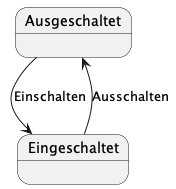
\includegraphics[width=0.25\textwidth]{fig/uml/lampe.png}
  \caption{Einfache FSM Lampe}
  \label{fig:lampe}
\end{figure}
Für die Erstellung einer geeigneten RESTful API mit HATEOAS (Hypermedia as the Engine of Application State) verwenden wir die folgende Struktur:
\\\\
Zustände abbilden:
\\
Ausgeschaltet: /lamp/off\\
Eingeschaltet: /lamp/on\\
\\\\
HTTP-Verben für Zustandsübergänge:
\\
Einschalten: PUT /lamp/on\\
Ausschalten: PUT /lamp/off
\\\\
Nun werden noch die HATEOAS-Links in den API-Antworten eingebunden. Somit ergibt sich ein Beispiel für eine JSON-Antwort, wenn die Lampe ausgeschaltet ist:\\\\
\noindent\begin{minipage}{\textwidth}
\begin{lstlisting}[caption={Fallbeispiel REST - aus},captionpos=b,label={lst:rest_on}]
{
  "state": "Ausgeschaltet",
  "links": [
    {
      "rel": "self",
      "href": "/lamp/off",
      "method": "GET"
    },
    {
      "rel": "Einschalten",
      "href": "/lamp/on",
      "method": "PUT"
    }
  ]
}
\end{lstlisting}
\end{minipage}

\noindent\begin{minipage}{\textwidth}
\begin{lstlisting}[caption={Fallbeispiel REST - an},captionpos=b,label={lst:rest_an}]
{
  "state": "Eingeschaltet",
  "links": [
    {
      "rel": "self",
      "href": "/lamp/on",
      "method": "GET"
    },
    {
      "rel": "Ausschalten",
      "href": "/lamp/off",
      "method": "PUT"
    }
  ]
}
\end{lstlisting}
\end{minipage}
Die JSON-Antworten enthalten den aktuellen Zustand der Lampe und HATEOAS-Links, die den möglichen Zustandsübergängen entsprechen. Dies ermöglicht es den Clients, die API dynamisch zu erkunden und zu verwenden, ohne die zugrunde liegende Struktur der API kennen zu müssen.\\\\

Liegt die Lösung der Software-Architektur als funktionale Zerlegung in der Grundarchitektur - beispielhaft - in einer MVC Architektur vor, könnte ein Adapter die Lücke zwischen der REST Architektur und der MVC Architektur schließen. Um einen Adapter zu erstellen, können wir das Adapter-Entwurfsmuster verwenden. Im Folgenden finden Sie ein Beispiel, das den vorherigen Ansatz modifiziert, um das MVC-Muster zu integrieren:


Um das Beispiel zu vereinfachen, wurde ein Python Syntax gewählt. Zuerst erstellen wir ein Lampenmodell, das die Logik für das Ein- und Ausschalten der Lampe enthält:\\\\
\noindent\begin{minipage}{\textwidth}
\begin{lstlisting}[caption={LampModel},captionpos=b,label={lst:lamp_m}]
class LampModel:
    def __init__(self):
        self.state = "AUS"

    def toggle(self):
        if self.state == "AUS":
            self.state = "EIN"
        else:
            self.state = "AUS"

    def get_state(self):
        return self.state

\end{lstlisting}
\end{minipage}
Dann erstellen wir einen Lampen-Controller, der das Modell verwendet und die Methoden on() und off() bereitstellt:\\\\
\noindent\begin{minipage}{\textwidth}
\begin{lstlisting}[caption={LampController},captionpos=b,label={lst:lamp_c}]
class LampController:
    def __init__(self, model):
        self.model = model

    def on(self):
        if self.model.get_state() == "AUS":
            self.model.toggle()

    def off(self):
        if self.model.get_state() == "EIN":
            self.model.toggle()
\end{lstlisting}
\end{minipage}
Schließlich erstellen wir einen Adapter, der den Lampen-Controller verwendet, um die Methoden on() und off() in der REST-API zu nutzen:\\\\
%\noindent\begin{minipage}{\textwidth}
\begin{lstlisting}[caption={LampAdapter},captionpos=b,label={lst:lamp_a}]
class LampAdapter(Resource):
    def __init__(self, controller):
        self.controller = controller

    def get(self):
        response = {
            "state": self.controller.model.get_state(),
            "_links": {
                "self": {"href": "/lamp"},
                "on": {"href": "/lamp/on"},
                "off": {"href": "/lamp/off"},
            }
        }
        return jsonify(response)

    def put(self):
        action = request.form.get("action")

        if action == "on":
            self.controller.on()
        elif action == "off":
            self.controller.off()

        response = {
            "state": self.controller.model.get_state(),
            "_links": {
                "self": {"href": "/lamp"},
                "on": {"href": "/lamp/on"},
                "off": {"href": "/lamp/off"},
            }
        }
        return jsonify(response)
\end{lstlisting}
%\end{minipage}
Zum Schluss integrieren wir den Adapter prototypisch in die Flask-App:\\\\
%\noindent\begin{minipage}{\textwidth}
\begin{lstlisting}[caption={Lamp REST APP},captionpos=b,label={lst:lamp_r}]
from flask import Flask, jsonify, request
from flask_restful import Resource, Api

app = Flask(__name__)
api = Api(app)

lamp_model = LampModel()
lamp_controller = LampController(lamp_model)
lamp_adapter = LampAdapter(lamp_controller)

api.add_resource(lamp_adapter, "/lamp", "/lamp/toggle", "/lamp/on", "/lamp/off")

if __name__ == "__main__":
    app.run(debug=True)
\end{lstlisting}
%\end{minipage}
Der Adapter verbindet nun das REST-Design mit dem MVC-Design. Die API unterstützt das Ein- und Ausschalten der Lampe über separate Endpunkte (/lamp/on und /lamp/off). Der Adapter verwendet den Lampen-Controller, um die on()- und off()-Methoden aufzurufen und auf das Modell zuzugreifen.
\\\\
Die vorgestellte Lösung ist ein Beispiel dafür, wie man das MVC-Design (Model-View-Controller) mit RESTful-APIs kombiniert, um sauberen und wartbaren Code zu schreiben. Es ist insofern üblich, als dass es bewährte Praktiken aus Software-Designmustern und Architekturen verwendet.

Es ist wichtig zu beachten, dass es keine \enquote{Einheitslösung} gibt, die auf alle Projekte oder Situationen anwendbar ist. Die beste Lösung hängt von den spezifischen Anforderungen und Bedingungen Ihres Projekts ab. In vielen Fällen ist es jedoch sinnvoll, Designmuster wie MVC und RESTful-APIs zu verwenden, um eine klare Trennung von Verantwortlichkeiten zu erreichen und die Komplexität des Codes zu reduzieren. Die ist nur ein Beispiel, das die Anwendung dieser Prinzipien zeigt und kann als Ausgangspunkt für die Anpassung an die Anforderungen Ihres Projekts dienen. In der Praxis müssen Sie möglicherweise verschiedene Aspekte wie Skalierbarkeit, Performance und Sicherheit berücksichtigen und auf zusätzliche Anforderungen und Herausforderungen reagieren, die sich aus der realen Anwendung ergeben.
\\\\
Dennoch, die ReSTful-API eignet sich in dem Sinne der funktionalen Zerlegung für eine Lampe, da wir eine zeitliche Kopplung mit einem zustandslosen Dienst vorfinden. Sollten wir aber eine Echtzeitanforderung an die Schaltung der Lampe über Best-Effort formulieren, oder an der Lampe noch einen Bewegungsmelder mit automatischer Aktivierung der Lampe montieren, wirkt die Lösung mit der vorgestellten RESTful API nicht mehr attraktiv. 
\\\\
Diskutierbar ist auch ein weiteres Beispiel mit einer noch loseren zeitlichen Kopplung als über RESTful API Alternativen, oder der Nutzung leichtgewichtigerer Lösungen.
Alternativen zu RESTful API können zum Beispiel sein
\begin{itemize}
\item \textbf{CoAP} (Constrained Application Protocol): CoAP ist ein leichtgewichtiges, webbasiertes Protokoll, das speziell für eingeschränkte Umgebungen und Geräte entwickelt wurde. Es basiert auf dem REST-Architekturstil und verwendet das User Datagram Protocol (UDP) statt TCP, was es für den Einsatz in Low-Power- und verlustbehafteten Netzwerken geeignet macht. CoAP unterstützt die gleichen HTTP-Methoden wie GET, POST, PUT und DELETE und bietet eine einfache Möglichkeit, Ressourcen in IoT-Anwendungen zu identifizieren und zu manipulieren.
\item \textbf{XMPP} (Extensible Messaging and Presence Protocol): XMPP ist ein offenes, XML-basiertes Protokoll, das ursprünglich für Instant Messaging und Präsenzinformationen entwickelt wurde. Es ist ein erweiterbares und flexibles Protokoll, das auch für IoT-Anwendungen verwendet werden kann. XMPP bietet eine Vielzahl von Funktionen, wie beispielsweise die Fähigkeit, Nachrichten an mehrere Empfänger zu senden, und es unterstützt die Kommunikation über verschiedene Netzwerktopologien hinweg.
\item \textbf{AMQP} (Advanced Message Queuing Protocol): AMQP ist ein offenes, binäres Messaging-Protokoll, das für die Kommunikation zwischen Anwendungen und Systemen entwickelt wurde. Es ist ein zuverlässiges und sicheres Protokoll, das verschiedene Nachrichtenaustauschmuster wie Publish-Subscribe, Punkt-zu-Punkt und Request-Reply unterstützt. Im Vergleich zu MQTT ist AMQP komplexer und bietet mehr Funktionen, was es für den Einsatz in Enterprise-Anwendungen und für den Nachrichtenaustausch in verteilten Systemen geeignet macht.
\item \textbf{DDS} (Data Distribution Service): DDS ist ein Echtzeit-Publish-Subscribe-Protokoll, das für die Verteilung und den Austausch von Daten in Hochleistungs- und Echtzeitanwendungen entwickelt wurde. Es bietet Funktionen wie Quality of Service (QoS), Filterung und Sicherheit und eignet sich besonders für Anwendungen in Industrie, Verteidigung und Luft- und Raumfahrt.
\item \textbf{OPC-UA} (OPC Unified Architecture): OPC-UA ist ein industrielles Kommunikationsprotokoll, das für den Datenaustausch zwischen industriellen Steuerungssystemen und Automatisierungsgeräten entwickelt wurde. Es ist ein plattformunabhängiges, skalierbares und sicheres Protokoll, das eine Vielzahl von Funktionen bietet, wie z. B. Informationsmodellierung, Sicherheit und Discovery.
\end{itemize}
Die Auswahl des am besten geeigneten Protokolls hängt von den spezifischen Anforderungen und Zielen des Projekts ab. Dabei sollten Faktoren wie Bandbreite, Latenz, Sicherheit, Skalierbarkeit und Netzwerkumgebung berücksichtigt werden. Eine immer größere Beliebtheit haben Message Queue Broker Protokolle, die nun in einem eigenen Kapitel diskutiert werden.  

\subsubsection{IETF Message Broker Protokolle}

AMQP, STOMP und MQTT sind alle Protokolle, die für die Nachrichtenübertragung zwischen Systemen und Geräten aus dem Kontext der IETF verwendet werden können. Sie sind auf unterschiedliche Weise gestaltet und bieten unterschiedliche Funktionen, aber sie haben auch einige Gemeinsamkeiten. Alle drei Protokolle sind zustandsbasiert, was bedeutet, dass sie eine Verbindung zwischen dem Client und dem Broker herstellen und aufrechterhalten, um die Nachrichtenübertragung zu erleichtern. Sie verwenden alle einen Broker als Vermittler zwischen den Clients, um die Nachrichtenübertragung zu koordinieren und zu verwalten.
Alle drei Protokolle unterstützen eine Vielzahl von Anwendungen und können in verschiedenen Umgebungen wie IoT, Messaging-Systemen und anderen Anwendungsfällen eingesetzt werden.
Sie bieten alle eine hohe Skalierbarkeit, um die Anforderungen an die Nachrichtenübertragung in großen Systemen und Netzwerken zu erfüllen. 
\\\\
\textbf{AMQP}, die Abkürzung für Advanced Message Queuing Protocol, wurde als offener Ersatz für bestehende proprietäre Messaging-Middleware entwickelt. Zwei der wichtigsten Gründe für die Verwendung von AMQP sind Zuverlässigkeit und Interoperabilität. Wie der Name schon andeutet, bietet es eine breite Palette von Funktionen für das Messaging, einschließlich zuverlässiger Warteschlangen, themenbasiertem Publish-and-Subscribe-Messaging, flexiblem Routing, Transaktionen und Sicherheit. AMQP-Austausche leiten Nachrichten direkt weiter. Dies geschieht nach Themen (Topics) oder auch basierend auf Header-Informationen.

Bei einem so umfangreichen Funktionsumfang sind viele fein abgestufte Steuerungsmöglichkeiten vorhanden. Sie können den Zugriff auf Warteschlangen beschränken, ihre Tiefe verwalten und vieles mehr. Funktionen über Nachrichteneigenschaften, Anmerkungen und Header machen es zu einer guten Lösung für eine Vielzahl von Unternehmensanwendungen. Dieses Protokoll wurde für die Steigerung der Zuverlässigkeit vieler großer Unternehmensanwendungen entwickelt, die auf Messaging angewiesen sind, um Anwendungen zu integrieren und Daten innerhalb ihrer Organisation zu bewegen. AMQP ist ein binäres Protokoll, das für die Interoperabilität zwischen verschiedenen Anbietern entwickelt wurde. Wo andere Protokolle versagt haben, hat sich AMQP durchgesetzt. Unternehmen wie JP Morgan verwenden es zur Verarbeitung von 1 Milliarde Nachrichten pro Tag. Die NASA verwendet es für Nebula Cloud Computing. Google verwendet es für die komplexe Ereignisverarbeitung. Es wird in einer der weltweit größten biometrischen Datenbanken verwendet, dem indischen Aadhar-Projekt, das 1,2 Milliarden Identitäten enthält. Es wird in der Ocean Observatories Initiative verwendet - eine Architektur, die täglich 8 Terabyte an Daten sammelt. 
\\\\
\textbf{MQTT} (Message Queue Telemetry Transport) wurde ursprünglich vom IBM-Team für Pervasive Computing und dessen Arbeit mit Partnern aus der Industrie entwickelt. In den letzten Jahren wurde das Protokoll in die Open-Source-Gemeinschaft überführt, erfuhr mit dem Aufschwung mobiler Anwendungen einen beträchtlichen Popularitätszuwachs. Die Konstruktionsprinzipien und Ziele von MQTT sind viel einfacher und zielgerichteter als die von AMQP - es bietet Publish-and-Subscribe-Messaging (keine Warteschlangen, trotz des Namens) und wurde speziell für ressourcenbeschränkte Geräte und Netzwerke mit geringer Bandbreite und hoher Latenz entwickelt. Im Grunde kann es besonders in eingebetteten Systemen effektiv eingesetzt werden.

Einer der Vorteile von MQTT gegenüber vollwertigen \enquote{Enterprise Messaging}-Brokern besteht darin, dass es aufgrund seines absichtlich geringen Platzbedarfs ideal für die heutigen mobilen und sich entwickelnden Anwendungen im Stil des \enquote{Internet der Dinge} ist. Unternehmen wie Facebook verwenden es sogar als Teil ihrer mobilen Anwendungen, weil es so wenig Strom verbraucht und die Netzwerkbandbreite schont.

Einige der MQTT-basierten Broker unterstützen viele tausend gleichzeitige Geräteverbindungen. MQTT bietet drei Dienstqualitäten.

Die Stärken von MQTT sind Einfachheit (nur fünf API-Methoden), eine kompakte binäre Paket-Nutzlast (keine Nachrichteneigenschaften, komprimierte Header, viel weniger ausführlich als etwas Textbasiertes wie HTTP), und es eignet sich gut für einfache Push-Nachrichten-Szenarien wie Temperatur-Updates, Börsenticker, Öldruck-Feeds oder mobile Benachrichtigungen. Es ist auch sehr nützlich, um Maschinen miteinander zu verbinden, z. B. um ein Arduino-Gerät mit einem Webdienst über MQTT zu verbinden.
\\\\
\textbf{STOMP} (Simple/Streaming Text Oriented Messaging Protocol) ist das einzige dieser drei Protokolle, das textbasiert ist und damit in Bezug auf sein Erscheinungsbild eher mit HTTP vergleichbar ist. Wie AMQP bietet STOMP einen Nachrichten- (oder Rahmen-) Header mit Eigenschaften und einen Rahmenkörper. Die Entwurfsprinzipien waren hier, etwas Einfaches und weitgehend Interoperables zu schaffen. So ist es beispielsweise möglich, eine Verbindung zu einem STOMP-Broker mit einem einfachen Telnet-Client herzustellen.

STOMP arbeitet jedoch nicht mit Warteschlangen und Themen, sondern verwendet eine SEND-Semantik mit einer \enquote{Ziel}-String. Der Broker muss auf etwas abbilden, das er intern versteht, wie z. B. ein Thema, eine Warteschlange oder einen Austausch. Die Verbraucher SUBSCRIBEN dann zu diesen Zielen. Da diese Ziele in der Spezifikation nicht vorgeschrieben sind, können verschiedene Broker unterschiedliche Arten von Zielen unterstützen. Daher ist es nicht immer einfach, Code zwischen Brokern zu portieren.

STOMP ist jedoch einfach und leichtgewichtig (wenn auch etwas langatmig auf dem Draht), mit einer breiten Palette von Sprachbindungen. Es bietet auch einige transaktionale Semantiken. Eines der interessantesten Beispiele ist RabbitMQ Web Stomp, mit dem Sie Nachrichten in einem Browser über Websockets bereitstellen können. Dies eröffnet einige interessante Möglichkeiten, z. B. die Aktualisierung eines Browsers, einer mobilen Anwendung oder einer Maschine in Echtzeit mit allen Arten von Informationen.

\subsubsection{Message Broker}
Das Skript legt im weiteren weniger Wert auf STOMP oder AMQP, sondern legt zunächst den Fokus auf MQTT und vergleicht es gegenüber einem proprietären Protokoll aus dem APACHE Kafka Kontext. MQTT steht für ein Beipiel bei der Unterstützung einer Vielzahl von Geräten und Apache Kafka für die Etablierung einer hohen Verarbeitung von einer Vielzahl von Transaktionen.
\\\\
MQTT (Message Queuing Telemetry Transport) und Apache Kafka sind zwei verschiedene Protokolle bzw. Systeme, die für die Kommunikation in verteilter Umgebung und für die Verarbeitung von Datenströmen entwickelt wurden. Sie haben unterschiedliche Anwendungsfälle und Eigenschaften. Hier ist eine Diskussion über die Hauptunterschiede zwischen MQTT und Kafka:
\\\\
MQTT ist wie erwähnt ein leichtgewichtiges Publish-Subscribe-Protokoll, das speziell für eingeschränkte Umgebungen und Geräte mit begrenzter Rechenleistung und Bandbreite entwickelt wurde. Apache Kafka hingegen ist ein verteiltes Streaming-System, das für die Verarbeitung großer Datenmengen und Hochdurchsatz-Workloads entwickelt wurde. Es ist ein skalierbares und fehlertolerantes System, das für die Kommunikation zwischen großen verteilten Anwendungen und für die Verarbeitung und Speicherung von Datenströmen in Echtzeit verwendet wird.
\\\\
Während MQTT für Szenarien entwickelt wurde, in denen eine geringe Latenz und geringer Bandbreitenverbrauch wichtig sind, ist Kafka für den Datenaustausch und die Verarbeitung in groß angelegten, verteilten Anwendungen und Systemen entwickelt worden.

MQTT bietet eine Quality of Service (QoS) für die Nachrichtenübertragung, die es ermöglicht, unterschiedliche Grade der Zuverlässigkeit und Garantien für die Nachrichtenübermittlung zu wählen. Auf der anderen Seite bietet Kafka starke Haltbarkeits- und Verarbeitungsgarantien, indem es eine replizierte, verteilte und fehlertolerante Architektur verwendet.
\paragraph{MQ Technologiestacks\\\\}
Auch Kafka, wenngleich sehr stark verbreitet ist in seinem Kontext - wie MQTT in seinem - ist nicht ohne Alternativen. Es gibt verschiedene alternative Technologien zu Apache Kafka, die für ähnliche Anwendungszwecke wie das Verarbeiten von Datenströmen und die Kommunikation in verteilten Systemen verwendet werden können. Einige der bekanntesten sind:
\begin{itemize}
\item Apache Pulsar: Apache Pulsar ist ein verteiltes Messaging-System und Event-Streaming-Plattform, die für hohe Skalierbarkeit, Durchsatz und niedrige Latenz entwickelt wurde. Pulsar bietet eine getrennte Architektur für Messaging und Speicherung, was es ermöglicht, den Durchsatz und die Speicherkapazität unabhängig voneinander zu skalieren. Pulsar unterstützt auch Funktionen wie Geo-Replikation und Multi-Tenancy und kann als Alternative zu Kafka für Anwendungsfälle in verteilten Systemen und Echtzeit-Datenverarbeitung verwendet werden.
\item NATS Streaming: NATS Streaming ist ein leichtgewichtiges, hochleistungsfähiges Messaging-System, das auf dem NATS-Core-Protokoll aufbaut und zusätzliche Funktionen für die Verarbeitung von Datenströmen bereitstellt. Es bietet Funktionen wie At-least-once-Delivery, Nachrichten-Acknowledgements und Nachrichten-Historie. NATS Streaming ist für seine Einfachheit und geringe Latenz bekannt und kann für Anwendungsfälle verwendet werden, in denen schnelle Nachrichtenübermittlung und Echtzeit-Verarbeitung erforderlich sind.
\item Amazon Kinesis: Amazon Kinesis ist ein vollständig verwalteter Streaming-Datendienst, der von AWS bereitgestellt wird. Kinesis ermöglicht das Sammeln, Verarbeiten und Analysieren von Echtzeit-Datenströmen und bietet Funktionen wie skalierbare Dateneingabe und automatische Skalierung. Kinesis ist gut in das AWS-Ökosystem integriert und kann für Anwendungsfälle verwendet werden, in denen Echtzeit-Datenverarbeitung, -analyse und -überwachung erforderlich sind.
\item Google Cloud Pub/Sub: Google Cloud Pub/Sub ist ein Messaging- und Event-Streaming-Dienst, der von Google Cloud bereitgestellt wird. Pub/Sub ermöglicht die asynchrone Kommunikation zwischen verteilten Systemen und unterstützt Publish-Subscribe- und Point-to-Point-Messaging-Muster. Es ist gut in das Google Cloud-Ökosystem integriert und bietet Funktionen wie At-least-once-Delivery und automatische Skalierung.
\end{itemize}

Tatsächlich sind in dieser Aufzählung Technologien und Protokolle vermischt, die für Messaging und Datenverarbeitung verwendet werden. Der Grund dafür ist, dass in vielen Anwendungsfällen wie verteilten Systemen und Echtzeit-Datenverarbeitung, die Technologien und Protokolle eng miteinander verknüpft sind und oft zusammen verwendet werden, um bestimmte Funktionen zu erreichen und somit kaum mehr zwischen dem Protokoll und der technologischen Umsetzung unterschieden wird. Dies trifft nicht zuletzt sogar für Kafka zu. 

Apache Kafka ist sowohl ein Protokoll als auch eine Technologie, die auf dem Protokoll basiert. Es ist ein Messaging- und Streaming-System, das auf seinem eigenen Protokoll aufbaut. Somit wurde - zum besseren Verständnis - in der Aufzählung nur versucht, alternative Technologien und Protokolle zu nennen, die auch ähnliche Anwendungsfälle wie Kafka abdecken können. Es ist jedoch wichtig, zwischen den Protokollen und den Technologien, die diese Protokolle implementieren, zu unterscheiden. Dies ist aber besser am Beispiel MQTT diskutiert.
\\\\
Gerade die Vielzahl der Umsetzung von Message Broker mit MQTT Unterstützung können selbst den geneigtesten Leser irritiert zurück lassen\footnote{\url{https://github.com/hobbyquaker/awesome-mqtt}}. Aus diesem sehr großen Kontext, können beispielhaft RabbitMQ und ZeroMQ genannt werden. RabbitMQ, ZeroMQ und andere Messaging-Lösungen bieten unterschiedliche Funktionen und Eigenschaften, die sie für verschiedene Anwendungsfälle und Umgebungen geeignet machen. Die Vielzahl von Message-Broker-Implementierungen existiert, weil es eine breite Palette von Anforderungen und Szenarien in verteilten Systemen und Echtzeit-Kommunikation gibt, die von verschiedenen Lösungen besser oder schlechter abgedeckt werden können.
\\\\
RabbitMQ ist ein Open-Source-Message-Broker, der neben dem MQTT auch das Advanced Message Queuing Protocol (AMQP) implementiert. Es unterstützt verschiedene Messaging-Szenarien wie Publish-Subscribe, Point-to-Point und Request-Reply. RabbitMQ ist für seine Robustheit, Zuverlässigkeit und Skalierbarkeit bekannt und eignet sich für Enterprise-Anwendungen und für den Einsatz in verteilten Systemen.
\\\\
ZeroMQ hingegen ist eine leichtgewichtige Messaging-Bibliothek, die für hohe Leistung und geringe Latenz optimiert ist. Im Gegensatz zu RabbitMQ, das als zentralisierter Broker fungiert, ist ZeroMQ brokerlos und ermöglicht den direkten Austausch von Nachrichten zwischen Anwendungen oder Prozessen. ZeroMQ bietet verschiedene Kommunikationsmuster wie Publish-Subscribe, Request-Reply und Pipeline. Es eignet sich für Anwendungsfälle, in denen schnelle Kommunikation, geringe Latenz und einfache Skalierbarkeit erforderlich sind.
\\\\
Wichtig ist aber zu verstehen, das bei der Vielzahl der Angebote die Grundarchitektur immer sehr ähnlich ist, das folgende Kapitel wird es exemplarisch diskutieren.

\subsubsection{Message Broker Architektur}

Die Wahl der richtigen Messaging-Lösung hängt von Faktoren wie Skalierbarkeit, Latenz, Zuverlässigkeit, Kommunikationsmuster und Integration in bestehende Infrastrukturen ab. Die Vielzahl von Message-Broker-Implementierungen ermöglicht es Entwicklern, die beste Lösung für ihre Anwendungsfälle auszuwählen, indem sie die spezifischen Anforderungen ihrer Projekte und die Eigenschaften der verfügbaren Messaging-Lösungen berücksichtigen. Durch das Verständnis der Unterschiede zwischen diesen Lösungen können Entwickler fundierte Entscheidungen über die Auswahl der richtigen Messaging-Technologie für ihre Projekte treffen. Das Bauchgefühl ist hier keine gute Entscheidungsgrundlage. 
\\\\
In dem bisherigen Text sind aus Sicht des Autors die neun wichtigsten - aufgrund ihrer Marktverbreitung und Popularität - Message Broker genannt worden, zur Vervollständigung einer - wenngleich nicht die - Top 10 kann noch die IBM MQ (früher WebSphere MQ) genannt werden. Ein proprietärer Message-Broker von IBM, der für seine Zuverlässigkeit, Sicherheit und Integration in IBM-Systeme und andere Enterprise-Anwendungen bekannt ist.
\\\\
Bei IBM MQ handelt es sich um einen Middleware-Service, der eine asynchrone und zuverlässige Nachrichtenübermittlung zwischen den Systemen gewährleistet und diese Eigenschaft mit den meisten der hier genannten Systemen teilt. Hier lohnt sich in der Diskussion insbesondere ein Blick auf die internen Komponenten, dass diese nicht selten und dabei nicht zu Letzt von \cite{tanenbaum2017distributed} als Referenz herangezogen werden.
\\\\
Die innere Architektur von IBM MQ besteht aus mehreren Komponenten, die zusammenarbeiten, um eine zuverlässige und sichere Nachrichtenübermittlung zu gewährleisten:

\begin{itemize}
\item Message Queues: IBM MQ verwendet Warteschlangen, um Nachrichten zwischen den Systemen zu übermitteln. Die Anwendungen senden und empfangen Nachrichten über diese Warteschlangen, die als Puffer für Nachrichten dienen. Dadurch können Anwendungen unabhängig voneinander arbeiten und Systemausfälle abfedern, ohne dass Nachrichten verloren gehen.
\item Message Channel Agents (MCAs): MCAs sind verantwortlich für die Übertragung von Nachrichten zwischen den MQ-Servern (auch als Queue-Managern bezeichnet). Sie sorgen dafür, dass die Nachrichten sicher und zuverlässig zwischen den Systemen übertragen werden, indem sie Funktionen wie Verschlüsselung, Komprimierung und Nachrichten-Acknowledgements bereitstellen.
\item Queue Manager: Der Queue Manager ist das Herzstück von IBM MQ und verwaltet die Warteschlangen und die Nachrichtenübermittlung. Er ist dafür verantwortlich, die Nachrichten zwischen den Warteschlangen zu übertragen, die Nachrichtenpersistenz sicherzustellen und die Verarbeitung von Nachrichten zu steuern.
\item Clients: IBM MQ Clients sind Anwendungen, die auf Client-Systemen ausgeführt werden und mit dem IBM MQ Server über das Message Queue Interface (MQI) kommunizieren. Die Clients senden und empfangen Nachrichten über die Warteschlangen und können in verschiedenen Programmiersprachen geschrieben sein.
\end{itemize}

Unter der Haube wird das Publish-Subscribe-Pattern in der Regel durch eine Message Queue implementiert. Der Publisher sendet die Nachrichten an eine Queue, die für die Empfänger zugänglich ist. Die Empfänger können sich auf die Queue abonnieren, um die Nachrichten zu erhalten, die vom Publisher gesendet werden. Sobald eine neue Nachricht in der Queue eintrifft, wird sie an alle Abonnenten der Queue verteilt.
\\\\
Das Pub-Sub-Muster kann auch durch andere Mechanismen implementiert werden, wie z.B. durch die Verwendung von Topics oder Channels. In diesem Fall sendet der Publisher die Nachrichten an einen bestimmten Topic oder Channel, und die Empfänger abonnieren den entsprechenden Topic oder Channel, um die Nachrichten zu erhalten.
\\\\
Es gibt verschiedene Möglichkeiten, die Priorisierung von Nachrichten in einer Publish-Subscribe-Architektur umzusetzen.

Eine Möglichkeit ist die Verwendung von Prioritätsniveaus, bei der jede Nachricht eine Priorität zugewiesen wird. Die Prioritäten können je nach der Bedeutung der Nachricht oder dem Zeitrahmen, innerhalb dessen sie verarbeitet werden muss, variiert werden. Die Message Queue kann dann so konfiguriert werden, dass sie die höher priorisierten Nachrichten zuerst verarbeitet.

Eine weitere Möglichkeit ist die Verwendung von Routing-Regeln, bei der die Nachrichten basierend auf bestimmten Kriterien an bestimmte Empfänger weitergeleitet werden. Diese Kriterien können beispielsweise der Inhalt der Nachricht, der Sender oder der Empfänger sein. Durch die Verwendung von Routing-Regeln können Nachrichten an die richtigen Empfänger weitergeleitet werden, basierend auf ihrer Priorität.

Es gibt auch spezialisierte Software-Tools, die die Priorisierung von Nachrichten in Publish-Subscribe-Systemen unterstützen. Zum Beispiel kann Apache Kafka Konfigurationen bereitstellen, um die Reihenfolge der Verarbeitung von Nachrichten zu steuern und das Verarbeiten von höher priorisierten Nachrichten zu priorisieren.

\subsubsection{Fehlersemantik}

Neben der Priorisierung ist auch die Qualität der Dienstleistung (QoS) entscheidend für den Erfolg, insbesondere die damit verbundenen Fehlersemantik. Dies soll am Beispiel von MQTT diskutiert werden.
MQTT unterstützt drei QoS-Levels (0, 1 und 2), die unterschiedliche Garantien bezüglich der Nachrichtenzustellung bieten. die im Folgenden  auch allgemeine diskutiert werden sollen. 
\begin{itemize}
\item QoS 0 - Maybe: QoS 0 bedeutet, dass Nachrichten nach Best Effort QoS zugestellt werden. Es gibt keine Garantie für die Zustellung, und es ist möglich, dass Nachrichten verloren gehen oder dupliziert werden. Dieses Level ist ideal für Anwendungsfälle, bei denen Datenverlust oder Duplikate tolerierbar sind, z. B. bei Sensordaten, die kontinuierlich übertragen werden. Die Fehlersemantik in diesem Level ist \enquote{maybe} (vielleicht), da die Zustellung nicht garantiert ist.
\item QoS 1 - At-least-once (Mindestens einmal):
Bei QoS 1 wird sichergestellt, dass Nachrichten mindestens einmal zugestellt werden. Dies bedeutet, dass der Sender die Nachricht wiederholt sendet, bis eine Empfangsbestätigung (ACK) vom Empfänger erhalten wird. Dieses Level ist ideal für Anwendungsfälle, bei denen die Zustellung wichtiger ist, und Datenverlust vermieden werden muss. Die Fehlersemantik in diesem Level ist \enquote{at-least-once"}(mindestens einmal), da Nachrichten möglicherweise mehrmals zugestellt werden.
\item QoS 2 - Exactly-once (Genau einmal):
QoS 2 garantiert, dass Nachrichten genau einmal zugestellt werden. Dieses Level stellt sicher, dass keine Nachrichten verloren gehen oder dupliziert werden. Um dies zu erreichen, wird ein Vier-Wege-Handshake-Verfahren zwischen Sender und Empfänger durchgeführt, das den Nachrichtenaustausch koordiniert. Dieses Level ist ideal für Anwendungsfälle, bei denen sowohl Datenverlust als auch Duplikate unzulässig sind, z. B. bei Steuerungs- oder Transaktionsdaten. Die Fehlersemantik in diesem Level ist \enquote{exactly-once} (genau einmal), da Nachrichten garantiert nur einmal zugestellt werden.
\end{itemize}

Die Fehlersemantiken at-least-once, at-most-once und exactly-once beziehen sich auf die Garantien, die ein Kommunikationssystem oder ein Protokoll hinsichtlich der Zustellung von Nachrichten bietet und können noch allgemein gesprochen um maybe erweitert werden. Sie haben einen signifikanten Einfluss auf die Architektur und das Verhalten von Systemen in Bezug auf Stateless- oder Stateful-Charakteristiken, Geschwindigkeit und Blockierungen:
\begin{itemize}
\item  Maybe (Vielleicht): Die maybe-Fehlersemantik bedeutet, dass die Nachrichtenzustellung nicht garantiert ist und Nachrichten möglicherweise verloren gehen können. Systeme, die diese Semantik verwenden, sind in der Regel stateless, da sie keine Informationen über den Zustand der Nachrichtenübermittlung speichern. Die Geschwindigkeit ist in der Regel hoch, da es keine zusätzlichen Schritte oder Wiederholungen zur Sicherstellung der Zustellung gibt. Da keine Blockierungen aufgrund von Zustellungsbestätigungen oder wiederholten Nachrichtenübermittlungen auftreten, ist die Kommunikation in solchen Systemen meist reibungslos.
\item At-most-once (Höchstens einmal): Die at-most-once-Fehlersemantik stellt sicher, dass Nachrichten höchstens einmal zugestellt werden. Ähnlich wie bei der maybe-Semantik sind Systeme, die diese Semantik verwenden, in der Regel stateless und schneller, da sie keine zusätzlichen Schritte zur Überprüfung der Nachrichtenzustellung durchführen. Diese Systeme können jedoch Nachrichten verlieren, sind aber vor Duplikaten geschützt. Blockierungen sind minimal, da keine Zustellungsbestätigungen erwartet werden.
\item At-least-once (Mindestens einmal): Die at-least-once-Fehlersemantik garantiert, dass Nachrichten mindestens einmal zugestellt werden. Systeme, die diese Semantik verwenden, sind in der Regel stateful, da sie den Zustand von Nachrichtenübermittlungen und Bestätigungen speichern müssen. Die Geschwindigkeit dieser Systeme kann aufgrund der zusätzlichen Schritte, wie dem Warten auf Empfangsbestätigungen (ACKs) und möglichen Wiederholungen, beeinträchtigt werden. Blockierungen können auftreten, wenn ein System auf Zustellungsbestätigungen wartet oder wiederholte Nachrichtenübermittlungen durchführt.
\item Exactly-once (Genau einmal): Die exactly-once-Fehlersemantik garantiert, dass Nachrichten genau einmal zugestellt werden. Systeme, die diese Semantik verwenden, sind stateful, da sie den Zustand von Nachrichtenübermittlungen, Bestätigungen und zusätzlichen Handshakes verwalten müssen. Die Geschwindigkeit dieser Systeme ist im Vergleich zu den anderen Semantiken am niedrigsten, da mehr Schritte und Kommunikationsaustausch erforderlich sind, um die exakte Zustellung zu gewährleisten. Blockierungen sind häufiger, da Systeme auf Handshakes und Bestätigungen warten, um den Nachrichtenübermittlungsprozess abzuschließen.
\end{itemize}
In verteilten Systemen ist die Exactly-Once-Fehlersemantik (auch bekannt als \enquote{Exactly Once Delivery} oder \enquote{Exactly Once Processing}) ein wichtiges Konzept, bei dem eine Nachricht genau einmal erfolgreich verarbeitet wird. Die Idee ist, dass Daten weder verloren gehen noch doppelt verarbeitet werden. In der Praxis ist die Exactly-Once-Fehlersemantik im eigentlichen Sinne jedoch unmöglich, da verteilte Systeme immer von Unsicherheiten und Unvorhersehbarkeiten betroffen sind.

Einige der Hauptgründe, warum die Exactly-Once-Fehlersemantik im eigentlichen Sinne unmöglich ist, sind:
\begin{itemize}
\item Zwei-Generäle-Problem: Das ist ein bekanntes Problem in der Informatik, das zeigt, dass es in verteilten Systemen keine Garantie dafür geben kann, dass zwei Parteien zuverlässig zu einer Übereinkunft kommen, wenn es Unsicherheiten bei der Kommunikation gibt (z.B. Nachrichtenverlust). Dies wird im folgenden Text auch nochmals intensiver diskutiert.
\item Unzuverlässige Kommunikation: Netzwerke können unzuverlässig sein, und es ist möglich, dass Nachrichten verloren gehen, beschädigt oder verzögert werden. Dies erschwert die Implementierung einer Exactly-Once-Fehlersemantik.
\item Unvorhersehbare Systemausfälle: Verteilte Systeme sind anfällig für Hardware- oder Softwareausfälle. Es ist schwierig, eine Exactly-Once-Fehlersemantik zu gewährleisten, wenn man nicht genau wissen kann, welche Komponenten ausfallen und wann dies geschehen könnte.
\end{itemize}
Trotz dieser Herausforderungen gibt es Protokolle wie MQTT (Message Queuing Telemetry Transport), die eine Exactly-Once-Fehlersemantik versprechen. Dies wird durch die Implementierung eines Mechanismus zur Kontrolle der Nachrichtenübermittlung erreicht. Es ist wichtig zu betonen, dass MQTT eine Annäherung an die Exactly-Once-Fehlersemantik bietet und in den Definitionen unterschieden wird zwischen  \textbf{message delivery} und \enquote{message processing}.\footnote{\url{https://exactly-once.github.io/posts/exactly-once-delivery/}}

\paragraph{Zwei-Generäle-Problem \\\\}
Das grundsätzliche Problem kann mit den Zwei-Generäle-Problem argumentiert werden. Das Two Generals' Problem, auch bekannt als das Byzantinische Generäle Problem, ist ein klassisches Problem in der Informatik und Kommunikationstheorie, dass sich mit der Frage der Koordination und Vertrauensbildung zwischen zwei Parteien befasst, die über einen unzuverlässigen Kommunikationskanal kommunizieren.
\\\\
Stellen Sie sich vor, es gibt zwei Generäle, General A und General B, die jeweils eine Armee kommandieren. Sie planen, eine feindliche Stadt anzugreifen und müssen sich auf den genauen Zeitpunkt des Angriffs einigen. Sie sind jedoch räumlich getrennt und können nur über Boten kommunizieren, die Nachrichten zwischen ihnen hin- und hertragen. Das Problem ist, dass der Kommunikationsweg durch das feindliche Gebiet führt und es eine Chance gibt, dass Boten abgefangen und ihre Nachrichten verloren gehen.

Um den Angriff erfolgreich durchzuführen, müssen sich beide Generäle auf den gleichen Zeitpunkt einigen und sicher sein, dass der andere General die Nachricht empfangen hat und mit dem Plan einverstanden ist. Wenn einer der Generäle angreift, während der andere sich zurückhält, wird der Angriff fehlschlagen und beide Armeen werden vermutlich besiegt werden.

Nehmen wir an, General A entscheidet sich für einen Angriffszeitpunkt und sendet einen Boten zu General B, um ihn über den Plan zu informieren. Es gibt jedoch keine Garantie, dass der Bote General B erreicht. Selbst wenn der Bote General B erreicht, wie kann General A sicher sein, dass die Nachricht erfolgreich zugestellt wurde?

Um dies zu bestätigen, könnte General B einen Boten zurückschicken, um zu bestätigen, dass er die Nachricht erhalten hat und mit dem Angriffszeitpunkt einverstanden ist. Aber was, wenn dieser bestätigende Bote verloren geht? Dann wird General A nicht wissen, ob General B die ursprüngliche Nachricht erhalten hat, und der Angriff wird gefährdet sein.

Das Two Generals' Problem zeigt, dass es in solchen Szenarien unmöglich ist, eine absolute Gewissheit der Koordination und Übereinstimmung zwischen den beiden Parteien zu erreichen, wenn der Kommunikationskanal unzuverlässig ist. Dieses Problem ist relevant für die Informatik, insbesondere in verteilten Systemen und Netzwerken, bei denen Kommunikationskanäle nicht immer zuverlässig sind und Knoten möglicherweise nicht vertrauenswürdig sind.
\\\\
In der Praxis verwenden verteilte Systeme und Netzwerke verschiedene Techniken, um den Grad der Koordination und Konsistenz zu erhöhen, wie z. B. Konsensalgorithmen (z. B. Paxos oder Raft) oder fehlertolerante Protokolle. Diese Protokolle werden noch in einem späteren Kapitel genauer diskutiert. wie es auch sei, diese Lösungen bieten jedoch auch keine absolute Garantie, sondern erhöhen lediglich die Wahrscheinlichkeit einer erfolgreichen Kommunikation und Koordination.

\paragraph{Exactly-Once-Fehlersemantik mit MQTT\\\\}

Es ist schwierig, eine exakte Wahrscheinlichkeitsberechnung für das Auftreten eines Fehlers bei der Exactly-Once-Fehlersemantik mit MQTT QoS 2 anzugeben, da dies von vielen Faktoren abhängt, wie zum Beispiel der Zuverlässigkeit des Netzwerks, der verwendeten Hardware und Software, sowie von Umweltbedingungen. Stattdessen können wir eine grobe Schätzung der Wahrscheinlichkeit solcher Fehler basierend auf einigen Annahmen diskutieren.

Angenommen, die Wahrscheinlichkeit, dass eine einzelne Nachricht während der Übertragung verloren geht, ist p (z.B. p = 0.001 oder 0.1 \%). Diese Wahrscheinlichkeit kann aufgrund von Netzwerkproblemen, Hardware- oder Softwareausfällen auftreten.

In einem QoS 2-Szenario gibt es vier Hauptnachrichten, die zwischen Sender und Empfänger (bzw. Broker) ausgetauscht werden: PUBLISH, PUBREC, PUBREL und PUBCOMP. Für den Exactly-Once-Fehlersemantik-Fehler muss eine dieser Nachrichten verloren gehen, während gleichzeitig der Wiederholungsmechanismus von MQTT versagt.

Die Wahrscheinlichkeit, dass eine dieser vier Nachrichten verloren geht, kann mit der Formel $1 - (1 - p)^4$ berechnet werden, da wir annehmen, dass die Wahrscheinlichkeiten unabhängig voneinander sind.
\\\\
Für p = 0,001 (0,1 \%) erhalten wir:
\\\\
$1 - (1 - 0.001)^4 \approx 0.00397$ oder $0.397 \%$
\\\\
Die Wahrscheinlichkeit, dass eine der vier Hauptnachrichten verloren geht, beträgt also etwa 0.397 \%. Dies ist jedoch noch nicht die endgültige Wahrscheinlichkeit für das Versagen der Exactly-Once-Fehlersemantik, da wir auch den Wiederholungsmechanismus von MQTT berücksichtigen müssen.

Angenommen, der Wiederholungsmechanismus funktioniert mit einer Zuverlässigkeit von q (z.B. q = 0.999 oder 99.9 \%). Die Wahrscheinlichkeit, dass der Wiederholungsmechanismus ebenfalls versagt, beträgt (1 - q).

Die kombinierte Wahrscheinlichkeit für das Versagen der Exactly-Once-Fehlersemantik ist dann die Wahrscheinlichkeit, dass eine der vier Nachrichten verloren geht, multipliziert mit der Wahrscheinlichkeit, dass der Wiederholungsmechanismus versagt:
\\\\
$0.00397 * (1 - 0.999) \approx 0.00000397 oder 0.000397 \%$
\\\\
In diesem Beispiel beträgt die Wahrscheinlichkeit, dass die Exactly-Once-Fehlersemantik versagt, etwa 0.000397 \%, wenn wir die oben genannten Annahmen treffen. Es ist wichtig zu betonen, dass diese Berechnung stark von den angenommenen Wahrscheinlichkeiten p und q abhängt und in der Praxis variieren kann.

Trotzdem zeigt das Beispiel, dass die Wahrscheinlichkeit eines Versagens der Exactly-Once-Fehlersemantik in einem gut konfigurierten MQTT-System mit QoS 2 sehr gering ist, solange die Netzwerk-, Hardware- und Softwarebedingungen zuverlässig sind.

Und somit ist es erwähnenswert, dass trotz solcher Ausnahmefälle MQTT mit QoS 2 eine hohe Zuverlässigkeit bei der Nachrichtenübermittlung bietet, indem es den Nachrichtenaustausch koordiniert und den Zustand der Nachrichten beibehält. Solche Szenarien sind extrem selten, und MQTT ist in der Regel in der Lage, die Exactly-Once-Fehlersemantik erfolgreich durchzuführen. Dennoch eine 100 \%-ige Sicherheit ist es nicht, dies wird uns auch nochmal zu einem späteren Zeitpunkt begleiten. 

\paragraph{Message Broker in der Praxis\\\\}

Bei Message Brokern werden oft einige Aspekte unterschätzt, die zu Herausforderungen führen können. Hier sind einige Beispiele:

\begin{itemize}
\item Komplexität: Die Einrichtung und Konfiguration eines Message Brokers kann sehr komplex sein. Es erfordert ein tiefes Verständnis der Funktionsweise des Brokers sowie der Anforderungen der Anwendung, die ihn nutzt.
\item Ausfallsicherheit: Da Message Broker oft eine zentrale Rolle in der Architektur einnehmen, müssen sie in der Regel sehr ausfallsicher sein. Ein Ausfall des Brokers kann schwerwiegende Folgen für die gesamte Anwendung haben.
\item Skalierbarkeit: Skalierbarkeit ist ein wichtiger Aspekt von Message Brokern. Wenn die Anzahl der Nachrichten oder der Verkehr auf der Plattform zunimmt, muss der Broker in der Lage sein, diese Last zu bewältigen.
\item Leistung: Die Leistung von Message Brokern ist ein weiterer wichtiger Aspekt, der oft unterschätzt wird. Wenn die Verarbeitungsgeschwindigkeit von Nachrichten nicht ausreicht, kann dies zu Verzögerungen in der Anwendung führen.
\item Sicherheit: Message Brokern müssen sicher sein, um sicherzustellen, dass vertrauliche oder sensible Informationen nicht in die falschen Hände geraten.
\item Kompatibilität: Da Message Broker in der Regel in verschiedenen Anwendungen und Systemen eingesetzt werden, muss die Kompatibilität mit anderen Systemen sichergestellt werden, um eine reibungslose Integration zu ermöglichen.
\item Wartung und Support: Die Wartung und Unterstützung von Message Brokern kann sehr zeitaufwändig sein. Es ist wichtig, sicherzustellen, dass der Broker regelmäßig gewartet und aktualisiert wird, um sicherzustellen, dass er sicher und zuverlässig bleibt.
\end{itemize}
Das führt wiederum zu neuen Geschäftsmodellen, wo die Nutzung des Message Brokers im Grunde verschenkt wird, um den Nutzer an die Serice Leistungen zu binden, die im besten Fall die Nachteile des Systems auffangen. 
Ein Beispiel ist hier HiveMQ. HiveMQ ist ein kommerzielles MQTT-Messaging-System, das auf die Implementierung von IoT-Plattformen und -Anwendungen spezialisiert ist. Das Unternehmen bietet sowohl eine Cloud-basierte als auch eine On-Premises-Version seines Produkts an und generiert Einnahmen durch den Verkauf von Lizenzen und den Abschluss von Abonnements.
\\\\
Das Hauptgeschäftsmodell von HiveMQ basiert auf der Lizenzierung seiner Messaging-Plattform an Unternehmen, die diese für ihre IoT-Anwendungen nutzen möchten. Es gibt verschiedene Lizenzierungsmodelle, die je nach den Anforderungen des Kunden angepasst werden können. Dazu gehören beispielsweise Abonnements auf Jahresbasis, die je nach der Anzahl der verbundenen Geräte oder der Anzahl der Nachrichten, die über die Plattform übertragen werden, gestaffelt sind.

HiveMQ bietet auch eine kostenlose Community-Version seiner Plattform an, die jedoch weniger Funktionen und Support bietet als die kommerzielle Version. 

Wichtig für den Erfolg eines Protokolls ist wie bereits öfter angesprochen das API Design. Am Ende entscheiden die Entwickler welche Technologie eingesetzt wird. So muss man verstehen, das somit häufig bei der Diskussion um die Anbindung weniger der Dienste und  die Protokolle wie HTTP, Kafka oder MQTT im Fokus stehen, sondern vielmehr der Zugriff auf die darin kodierten Funktionen. Diesen Ansatz mag man belächeln, er hat aber leider einen hohen Praxisbezug.  
\\\\
In der bekannten Fallarchitektur soll nochmals demonstriert werden, wie einfach eine Message Broker APi am Beispiel von MQTT sein kann. Es gibt drei Hauptkomponenten, die am etablierten Lampen-Fallbeispiel diskutiert werden sollen: den MQTT-Broker, den Lampen-Controller (Subscriber) und den Schalter (Publisher). Der MQTT-Broker fungiert als zentrale Kommunikationsschnittstelle und leitet Nachrichten zwischen den Clients weiter. Der Lampen-Controller und der Schalter sind MQTT-Clients, die sich mit dem Broker verbinden, um Nachrichten zu senden und zu empfangen.

Der Lampen-Controller ist ein IoT-Gerät, das die Lampe steuert. Es abonniert ein MQTT-Topic, zum Beispiel "lamp/control", und reagiert auf eingehende Nachrichten, indem es den Zustand der Lampe entsprechend ändert. Wenn der Controller eine Nachricht mit dem Inhalt \enquote{on} empfängt, schaltet er die Lampe ein, und wenn er eine Nachricht mit dem Inhalt \enquote{off} empfängt, schaltet er die Lampe aus.

Der Schalter ist ein weiteres IoT-Gerät oder eine Anwendung, die zum Steuern der Lampe verwendet wird. Wenn der Benutzer die Lampe ein- oder ausschalten möchte, sendet der Schalter eine entsprechende Nachricht (entweder \enquote{on} oder \enquote{off}) an das \enquote{lamp/control}-Topic.

Vorteile und Nachteile dieser Architektur: 
\begin{itemize}
\item Skalierbarkeit: Da das MQTT-Protokoll auf dem Publish/Subscribe-Modell basiert, können problemlos mehrere Lampen-Controller und Schalter hinzugefügt werden, ohne dass eine Änderung an der zugrunde liegenden Infrastruktur erforderlich ist.
\item Entkopplung: Die Verwendung eines zentralen Brokers entkoppelt die Lampen-Controller und Schalter voneinander, sodass sie unabhängig voneinander entwickelt, getestet und gewartet werden können.
\item Effizienz: MQTT ist ein leichtgewichtiges Protokoll, das sich gut für IoT-Anwendungen und den Einsatz in ressourcenbeschränkten Umgebungen eignet.
\item Qualität der Dienstleistung (QoS): MQTT unterstützt unterschiedliche QoS-Levels, die es ermöglichen, den Nachrichtenaustausch entsprechend den Anforderungen der Anwendung anzupassen.
\item Abhängigkeit von einem zentralen Broker: Ein zentraler Broker stellt einen Single Point of Failure dar, der die gesamte Kommunikation beeinträchtigen kann, wenn er ausfällt. Um dies zu vermeiden, können jedoch redundante Broker und Clustering-Lösungen eingesetzt werden.
\item Sicherheit: Die Sicherheit von MQTT muss durch die Implementierung von Authentifizierung, Autorisierung und Verschlüsselung (z.B. durch TLS) gewährleistet werden. Dies kann zusätzliche Komplexität und Overhead verursachen.
\item Latenz: Obwohl MQTT für Low-Bandwidth- und High-Latency-Netzwerke entwickelt wurde, kann es in einigen Situationen, insbesondere bei sehr großen oder überlasteten Netzwerken, zu Latenzproblemen kommen.
\end{itemize}

Generell ist eine Architektur mit MQTT zur Steuerung einer Lampe geeignet, wenn keine harten oder weichen Echtzeitanforderungen gestellt werden. Insbesondere wenn eine skalierbare Lösung benötigt wird, die eine große Anzahl von Lampen und Schaltern unterstützt ist MQTT RESTful APIs vorzuziehen, wenn die Infrastrukturkomponenten dies zulassen. 
Neben MQTT gibt es auch weitere Systeme die sich darauf optimiert haben Nachrichtenaustausch zwischen technischen Systemen zu realisieren. Eines ist das pub-sub Verfahren in ROS. 
\paragraph{Robot Operation System\\\\}
Robot Operating System (ROS) ist ein flexibles Framework für die Entwicklung von Software für Roboter. Es bietet eine Sammlung von Tools, Bibliotheken und Konventionen, die die Komplexität der Robotik-Entwicklung reduzieren und die Zusammenarbeit zwischen Entwicklern erleichtern. ROS ermöglicht es, modulare und wiederverwendbare Softwarekomponenten für Roboter zu erstellen, die auf verschiedenen Hardwareplattformen ausgeführt werden können.

Ein wichtiger Aspekt von ROS ist das Publish-Subscribe-Verfahren (auch bekannt als \enquote{pub-sub}), das die Kommunikation zwischen verschiedenen Softwarekomponenten (auch \enquote{Knoten} genannt) ermöglicht. Im pub-sub-Modell veröffentlichen Knoten Informationen in Form von Nachrichten auf sogenannten \enquote{Topics}. Andere Knoten, die an diesen Informationen interessiert sind, können diese Topics abonnieren und die veröffentlichten Nachrichten empfangen. Dieses Verfahren ermöglicht eine lose Kopplung zwischen den Knoten, da sie nicht direkt miteinander kommunizieren müssen und keine Kenntnis voneinander haben müssen.

Ein Beispiel für das Publish-Subscribe-Verfahren in ROS könnte ein Roboter sein, der aus verschiedenen Sensoren, Aktuatoren und Steuerungskomponenten besteht. Ein Sensor könnte seine Messdaten auf einem Topic veröffentlichen, während ein Steuerungsknoten dieses Topic abonniert, um auf Basis dieser Messdaten Entscheidungen zu treffen. Gleichzeitig kann der Steuerungsknoten Befehle auf einem anderen Topic veröffentlichen, das von den Aktuatoren abonniert wird, um den Roboter entsprechend zu steuern.
\\\\
In verteilten Systemen wie ROS ist die Synchronisation der Zeit zwischen den Knoten entscheidend, um eine konsistente und korrekte Kommunikation und Steuerung zu gewährleisten. Hier kommt das Network Time Protocol (NTP) ins Spiel. NTP ist ein Protokoll zur Synchronisation der Uhren von Computern in einem Netzwerk. Es ermöglicht es, die Systemzeit der Knoten in einem ROS-System aufeinander abzustimmen, um sicherzustellen, dass alle Knoten eine gemeinsame Zeitbasis haben.

Die Bedeutung von NTP in einem ROS-System liegt in seiner Fähigkeit, Zeitstempel für veröffentlichte Nachrichten bereitzustellen, die von anderen Knoten verwendet werden können, um die zeitliche Reihenfolge der Ereignisse zu bestimmen und möglicherweise verzögerte oder veraltete Nachrichten zu erkennen. Zeitstempel sind auch wichtig für die Koordination und Synchronisation von Aktionen zwischen verschiedenen Knoten, z. B. wenn mehrere Sensoren und Aktuatoren zusammenarbeiten müssen, um eine gemeinsame Aufgabe auszuführen. NTP werden wir im nächsten Kapitel nochmals ausführlicher behandeln. 
\\\\
ROS überwacht aber durch diese Struktur und die lose Kopplung nicht die Integrität, es werden aber Mechanismen, wie z.B. Heartbeats angeboten um dies zu realisieren.  In ROS werden Heartbeats nicht direkt vom Framework selbst implementiert, sondern sie können durch individuelle Knoten oder Pakete realisiert werden.
\\\\
Heartbeats sind essenzielle Mechanismen für die Kommunikation und Synchronisation in solchen Systemen und tragen zur Stabilität und Zuverlässigkeit bei. Im Folgenden werden verschiedene Aspekte von Heartbeats und ihre Rolle in verschiedenen Anwendungsszenarien diskutiert. 

\subsubsection{Heartbeat}

Ein Heartbeat ist ein periodisches Signal, das von einer Komponente eines verteilten Systems an andere Komponenten gesendet wird, um ihre  Verfügbarkeit und Erreichbarkeit zu signalisieren. Diese Signale dienen als Lebenszeichen, ähnlich dem menschlichen Herzschlag, und ermöglichen den Komponenten, den aktuellen Zustand des Systems zu überwachen und auf Veränderungen oder Störungen zu reagieren.
\\\\
Heartbeats in verteilten Systemen haben mehrere Funktionen, die für die Kommunikation und Synchronisation zwischen den Komponenten von Bedeutung sind:

\begin{itemize}
\item Fehlererkennung: Durch den regelmäßigen Austausch von Heartbeat-Signalen können die Komponenten eines verteilten Systems den Zustand ihrer Nachbarn überwachen. Wenn ein Heartbeat von einer Komponente für eine bestimmte Zeit nicht empfangen wird, kann dies auf einen Ausfall oder eine Fehlfunktion hindeuten. Die anderen Komponenten können dann Maßnahmen ergreifen, um den Ausfall zu beheben oder die betroffene Komponente zu ersetzen.
\item Synchronisation: In verteilten Systemen ist die Synchronisation von Prozessen und Aktionen von großer Bedeutung. Heartbeats können verwendet werden, um eine gemeinsame Zeitbasis für alle Komponenten zu etablieren, indem sie beispielsweise Zeitstempel in den gesendeten Signalen enthalten. Dies ermöglicht es den Komponenten, ihre Aktionen aufeinander abzustimmen und zeitliche Inkonsistenzen zu vermeiden.
\item Lastverteilung: Heartbeats können auch zur Überwachung der Auslastung der einzelnen Komponenten in einem verteilten System verwendet werden. Indem sie Informationen über ihre aktuelle Arbeitslast in den Heartbeat-Signalen übermitteln, können die Komponenten eine effektive Lastverteilung erreichen und sicherstellen, dass Ressourcen im System optimal genutzt werden.
\end{itemize}
Trotz ihrer weit verbreiteten Anwendung und Nützlichkeit haben Heartbeats jedoch einige Nachteile in verteilten Systemen. Zum einen erzeugen Heartbeats zusätzlichen Netzwerkverkehr, da sie in regelmäßigen Abständen zwischen den Knoten im System ausgetauscht werden müssen. In großen verteilten Systemen oder bei hoher Heartbeat-Frequenz kann dies zu einer signifikanten Belastung des Netzwerks führen, die die Leistung des gesamten Systems beeinträchtigen kann. Auch kann es aufgrund von Netzwerklatenz oder temporären Verbindungsproblemen vorkommen, dass Heartbeat-Nachrichten verspätet oder gar nicht ankommen. In solchen Fällen könnte das System fälschlicherweise annehmen, dass ein Knoten ausgefallen ist, obwohl dieser tatsächlich noch aktiv ist. Diese Fehlalarme können zu unnötigen Neustarts oder Umschaltungen in der Systemkonfiguration führen.
In sehr großen verteilten Systemen kann die Verwaltung und Überwachung von Heartbeats für alle Knoten eine Herausforderung darstellen.
Die Probleme von nicht verlässlichen Fehlerdedektoren werden zu einem späteren Zeitpunkt nochmal aufgenommen. 
\\\\
Die Skalierbarkeit von Heartbeat-basierten Überwachungssystemen kann durch die zunehmende Anzahl von Knoten und den damit verbundenen Verwaltungsaufwand beeinträchtigt werden. Weiter bieten Heartbeats nur grundlegende Informationen über den Status eines Knotens, nämlich ob er aktiv ist oder nicht. Sie liefern keine detaillierten Informationen über die Leistung oder den Zustand des Knotens. Für eine umfassendere Überwachung und Fehlerbehebung sind möglicherweise zusätzliche Mechanismen erforderlich.
Nicht zu Letzt ist die  Einrichtung und Konfiguration von Heartbeats, insbesondere in komplexen verteilten Systemen, zeitaufwändig und fehleranfällig. Außerdem erfordert die Verwendung von Heartbeats eine kontinuierliche Wartung und Anpassung der Heartbeat-Intervalle und Timeout-Werte, um eine optimale Systemleistung sicherzustellen. 
Heartbeats sind aber selten mit vielen Alternativen bestückt, sodass trotz all dieser Nachteile Heartbeats mit ergänzenden Methoden zur Überwachung der Verfügbarkeit von Knoten in verteilten Systemen eingesetzt werden. 

Im Folgenden werden verschiedene Arten von Heartbeat-Protokollen und Algorithmen vorgestellt und diskutiert, um ein tieferes Verständnis ihrer Funktionsweise und Anwendungsbereiche zu vermitteln.
\\\\
Zentralisierte Heartbeat-Protokolle sind auf eine zentrale Komponente oder einen zentralen Koordinator angewiesen, der für die Überwachung der Verfügbarkeit der Systemknoten verantwortlich ist. Diese zentrale Einheit erhält regelmäßige Statusmeldungen von den Knoten, um ihre Aktivität zu verfolgen. Im Falle eines Ausfalls oder einer nicht erhaltenen Statusmeldung von einem Knoten ergreift die zentrale Einheit entsprechende Maßnahmen, um das System zu stabilisieren. Allerdings weisen zentralisierte Heartbeat-Protokolle eine potenzielle Schwachstelle auf, da die zentrale Einheit selbst ausfallen oder überlastet sein kann, was zu einer Beeinträchtigung der Überwachungsfunktion führt.
\\\\
Ein praktisches Beispiel für ein zentralisiertes Heartbeat-Protokoll ist das Manager-Worker-Modell. In diesem Szenario gibt es einen zentralen Manager, der die Verfügbarkeit mehrerer Worker-Knoten überwacht. Die Nachrichtensequenz ist wie folgt:
\begin{enumerate}[label=(\alph*)]
\item Der Manager sendet periodisch Anfragen an die Worker-Knoten.
\item Die Worker-Knoten antworten mit Heartbeat-Nachrichten, um ihre Verfügbarkeit zu signalisieren.
\item Der Manager überwacht die empfangenen Heartbeat-Nachrichten und identifiziert ausgefallene Knoten, wenn keine Antwort innerhalb einer bestimmten Zeitspanne eintrifft.
\end{enumerate}

Im Gegensatz dazu basieren dezentralisierte Heartbeat-Protokolle auf einem peer-to-peer-Ansatz, bei dem jeder Knoten direkt mit seinen Nachbarn kommuniziert, um den Systemzustand zu überwachen. Dadurch werden Single Points of Failure vermieden, was zu einer erhöhten Fehlertoleranz und Robustheit führt. Diese Art von Protokollen ist gut geeignet für große, dynamische Systeme, bei denen Knoten häufig hinzugefügt oder entfernt werden.

Ein Beispiel für ein dezentralisiertes Heartbeat-Protokoll ist das Ring-Topologie-Modell. Die Knoten sind in einem Ring angeordnet, und jeder Knoten überwacht die Verfügbarkeit seines direkten Nachbarn. Die Nachrichtensequenz ist wie folgt:
\begin{enumerate}[label=(\alph*)]
\item Jeder Knoten sendet periodisch Heartbeat-Nachrichten an seinen direkten Nachbarn im Ring.
\item Die Knoten überwachen die empfangenen Heartbeat-Nachrichten und identifizieren ausgefallene Nachbarn, wenn keine Antwort innerhalb einer bestimmten Zeitspanne eintrifft.
\end{enumerate}

Eine weitere interessante Kategorie ist die der hierarchischen Heartbeat-Protokolle, bei denen die Knoten in einer hierarchischen Struktur organisiert sind. Die Überwachung der Verfügbarkeit erfolgt hier auf verschiedenen Ebenen, wobei übergeordnete Knoten die Verantwortung für die Überwachung einer Gruppe von untergeordneten Knoten übernehmen. Dies reduziert die Kommunikationslast, da die Anzahl der übermittelten Statusmeldungen verringert wird, und verbessert die Skalierbarkeit des Systems.

Ein praktisches Beispiel für ein hierarchisches Heartbeat-Protokoll ist ein Cluster-basiertes System. In diesem Szenario sind die Knoten in Cluster-Gruppen organisiert, wobei jeder Cluster einen Cluster-Manager hat. Die Nachrichtensequenz ist wie folgt:
\begin{enumerate}[label=(\alph*)]
\item Cluster-Manager senden periodisch Heartbeat-Anfragen an die Knoten innerhalb ihrer Cluster.
\item Die Knoten antworten mit Heartbeat-Nachrichten, um ihre Verfügbarkeit zu signalisieren.
\item Cluster-Manager überwachen die empfangenen Heartbeat-Nachrichten und identifizieren ausgefallene Knoten.
\item Cluster-Manager senden periodisch Statusberichte an einen übergeordneten Manager.
\item Der übergeordnete Manager überwacht die Statusberichte und erkennt ausgefallene Cluster-Manager.
\end{enumerate}

Gossip-basierte Heartbeat-Protokolle stellen eine weitere Alternative dar, die auf einer stochastischen Informationsverbreitung basiert. Bei diesen Protokollen teilen die Knoten ihre Statusinformationen in Form von \enquote{Gossip} oder Gerüchten mit einer begrenzten Anzahl von zufällig ausgewählten Nachbarn. Diese Nachbarn verbreiten die Informationen dann weiter, sodass das Wissen über den Systemzustand schließlich über das gesamte Netzwerk verbreitet wird. Dieses Vorgehen ermöglicht eine schnelle und effiziente Informationsverteilung, selbst in sehr großen und dynamischen Systemen, und bietet eine hohe Fehlertoleranz.

Ein praktisches Beispiel für ein Gossip-basiertes Heartbeat-Protokoll ist das SWIM-Protokoll (Scalable Weakly-consistent Infection-style Process Group Membership). In diesem Szenario verbreiten die Knoten ihre Verfügbarkeit über Gossip-Nachrichten. Die Nachrichtensequenz ist wie folgt:
\begin{enumerate}[label=(\alph*)]
\item Jeder Knoten wählt zufällig einen anderen Knoten aus und sendet ihm eine Heartbeat-Nachricht.
\item Der ausgewählte Knoten aktualisiert seine Mitgliederliste und wählt zufällig weitere Knoten aus, um die empfangene Heartbeat-Nachricht weiterzuleiten.
\item Dieser Prozess wird mehrmals wiederholt, bis die Informationen über die Verfügbarkeit der Knoten im gesamten Netzwerk verbreitet sind.
Knoten, die innerhalb einer bestimmten Zeitspanne keine Heartbeat-Nachricht von einem bestimmten Knoten erhalten, identifizieren diesen als ausgefallen und aktualisieren ihre Mitgliederliste entsprechend.
\end{enumerate}

Zentralisierte Heartbeat-Protokolle bieten eine einfache und leicht verständliche Implementierung, können jedoch bei Ausfall der zentralen Einheit anfällig sein. Dezentralisierte Heartbeat-Protokolle hingegen bieten eine höhere Fehlertoleranz durch ihren peer-to-peer-Ansatz, können jedoch unter Umständen eine erhöhte Kommunikationslast verursachen.

Hierarchische Heartbeat-Protokolle bieten eine gute Balance zwischen Skalierbarkeit und Robustheit, indem sie die Kommunikationslast über verschiedene Ebenen verteilen, während gossip-basierte Heartbeat-Protokolle die stochastische Informationsverbreitung nutzen, um eine effiziente und zuverlässige Überwachung auch in großen und dynamischen Systemen zu gewährleisten.
\\\\
Bei der Implementierung von Heartbeat-Protokollen und -Algorithmen in verteilten Systemen gibt es wichtige Aspekte zu berücksichtigen, einschließlich der Unterscheidung zwischen In-Band- und Out-of-Band-Kommunikation sowie der Priorisierung von Heartbeat-Prozessen. Darüber hinaus gibt es weitere Faktoren, die bei der Implementierung und dem Betrieb von Heartbeat-Protokollen beachtet werden müssen. Eine einzelne Betrachtung wird folgend beschrieben:

\begin{itemize} 
\item In-Band- und Out-of-Band-Kommunikation: In-Band-Kommunikation bedeutet, dass die Heartbeat-Nachrichten über den gleichen Kanal wie die reguläre Datenkommunikation im verteilten System übertragen werden. Dies kann zu einer zusätzlichen Last auf dem Kommunikationskanal führen und möglicherweise die Leistung des Systems beeinträchtigen. Um solche Probleme zu vermeiden, ist es wichtig, die Häufigkeit der Heartbeat-Nachrichten angemessen zu wählen und möglicherweise die Größe der Nachrichten zu reduzieren, um die Auswirkungen auf die reguläre Datenkommunikation zu minimieren. Out-of-Band-Kommunikation hingegen bedeutet, dass die Heartbeat-Nachrichten über separate Kanäle von der regulären Datenkommunikation übertragen werden. Dies kann dazu beitragen, die Leistungseinbußen zu vermeiden, die durch In-Band-Kommunikation verursacht werden könnten. Bei der Implementierung von Out-of-Band-Kommunikation ist es wichtig, dedizierte Kanäle oder Netzwerkverbindungen bereitzustellen, die ausschließlich für die Übertragung von Heartbeat-Nachrichten genutzt werden.
\item Priorisierung von Heartbeat-Prozessen: Die Priorisierung von Heartbeat-Prozessen ist entscheidend, um sicherzustellen, dass die Überwachung der Knotenverfügbarkeit nicht von anderen Prozessen im verteilten System beeinträchtigt wird. Es ist ratsam, die Heartbeat-Prozesse so einzustellen, dass sie unabhängig von der Last auf dem System regelmäßig ausgeführt werden. Dies kann beispielsweise durch die Verwendung von Echtzeit-Prioritäten oder durch die Zuteilung von dedizierten Ressourcen für die Heartbeat-Prozesse erreicht werden.
\item Fehlertoleranz und Wiederherstellung: Bei der Implementierung von Heartbeat-Protokollen ist es wichtig, Mechanismen zur Fehlererkennung und Wiederherstellung zu berücksichtigen, die dazu beitragen, die Stabilität und Zuverlässigkeit des Systems aufrechtzuerhalten. Dies kann beispielsweise durch redundante Kommunikationspfade, automatische Neustarts oder Datenreplikation erreicht werden.
\item Anpassungsfähigkeit: Da verteilte Systeme oft dynamisch sind und sich im Laufe der Zeit verändern, sollte die Implementierung von Heartbeat-Protokollen flexibel und anpassungsfähig sein, um Änderungen in der Systemkonfiguration oder in den Anforderungen bewältigen zu können. Es sollte ein besonderer Wert auf die Policy des Mechanismus gelegt werden. ei der Implementierung von Heartbeat-Protokollen ist es wichtig, ein effektives Konfigurationsmanagement bereitzustellen, das die Einstellung von Parametern wie Heartbeat-Intervallen, Timeouts und anderen Konfigurationsdetails ermöglicht. Dies erleichtert die Anpassung des Systems an verschiedene Anforderungen und Betriebsumgebungen.
\item Skalierbarkeit: Bei der Implementierung von Heartbeat-Protokollen ist es wichtig, die Skalierbarkeit des Systems zu berücksichtigen. Dies beinhaltet die Fähigkeit, die Anzahl der Knoten und Ressourcen im System effektiv zu verwalten, während die Leistung und Stabilität aufrechterhalten werden. Bei der Auswahl und Implementierung von Heartbeat-Protokollen sollten Skalierungsaspekte wie Kommunikationslast, Anzahl der Knoten und deren Organisation berücksichtigt werden.
\item Sicherheit: Bei der Implementierung von Heartbeat-Protokollen ist es wichtig, Sicherheitsaspekte zu berücksichtigen, um das System vor Angriffen oder Missbrauch zu schützen. Dies kann beispielsweise durch die Verwendung von Verschlüsselung, Authentifizierung und Autorisierung bei der Übertragung von Heartbeat-Nachrichten erreicht werden.
\item Monitoring und Logging: Um die Leistung und Zuverlässigkeit von Heartbeat-Protokollen im verteilten System zu überwachen, sollten umfangreiche Monitoring- und Logging-Funktionen bereitgestellt werden. Dies ermöglicht es, Probleme frühzeitig zu erkennen und gegebenenfalls Maßnahmen zur Behebung von Problemen oder zur Verbesserung der Leistung zu ergreifen
\end{itemize} 

Heartbeat-Protokolle und Selbstheilungskonzepte sind eng miteinander verbunden, da sie beide zur Erhaltung der Stabilität und Verfügbarkeit in verteilten Systemen beitragen. Watchdog-Patterns sind ebenfalls relevant, da sie eine Überwachungsfunktion für Systemkomponenten bieten und bei Fehlern eingreifen können. Im Folgenden wird der Zusammenhang zwischen diesen Konzepten genauer erläutert.
\\\\
Heartbeat-Protokolle können dazu genutzt werden, um automatische Wiederherstellungsmaßnahmen einzuleiten, wenn ein Knotenausfall oder eine Fehlfunktion erkannt wird. Selbstheilung in verteilten Systemen bezieht sich auf die Fähigkeit des Systems, auf Ausfälle oder Fehlfunktionen von Knoten zu reagieren und sich automatisch zu erholen, ohne dass eine manuelle Intervention erforderlich ist. Einige der Selbstheilungsstrategien umfassen Neustarts, Ressourcen-Neuzuweisungen, Datenreplikation und Neukonfiguration von Knoten. Heartbeat-Protokolle sind ein wesentlicher Bestandteil solcher Selbstheilungsmechanismen, da sie die benötigten Informationen über den Zustand der Knoten liefern und Ausfälle oder Fehlfunktionen frühzeitig erkennen.
\\\\
Watchdogs überwachen die Systemkomponenten und können bei Bedarf Korrekturmaßnahmen ergreifen, wie zum Beispiel das Neustarten eines ausgefallenen Knotens oder das Senden von Benachrichtigungen an Administratoren. In verteilten Systemen kann ein Watchdog in Kombination mit Heartbeat-Protokollen verwendet werden, um die Knotenverfügbarkeit und -leistung kontinuierlich zu überwachen. Wenn ein Knoten keine Heartbeat-Nachricht innerhalb eines festgelegten Zeitrahmens sendet oder empfängt, kann der Watchdog den Knoten als ausgefallen betrachten und entsprechende Selbstheilungsmaßnahmen einleiten.
\\\\
In der Zukunft könnten adaptive und lernende Heartbeat-Systeme eine zunehmend wichtige Rolle in verteilten Systemen spielen. Diese Systeme sind in der Lage, sich automatisch an Veränderungen in der Systemumgebung oder den Anforderungen anzupassen, um die Effizienz, Stabilität und Skalierbarkeit zu verbessern.

Ein zentraler Aspekt der zukünftigen Entwicklung von adaptiven und lernenden Heartbeat-Systemen ist die Integration von maschinellem Lernen und künstlicher Intelligenz. Indem sie maschinelles Lernen und künstliche Intelligenz einsetzen, können Heartbeat-Systeme Muster und Zusammenhänge in den gesammelten Daten erkennen und daraus lernen, um ihre Leistung und Effizienz zu optimieren. Zum Beispiel könnten sie die optimalen Heartbeat-Intervalle basierend auf der erkannten Systemlast oder der Anzahl der Knoten dynamisch anpassen.
\\\\
Ein weiterer wichtiger Aspekt der zukünftigen Entwicklung von adaptiven und lernenden Heartbeat-Systemen ist die zunehmende Vernetzung und Heterogenität von verteilten Systemen. Mit dem Aufkommen von Edge-Computing, dem Internet der Dinge (IoT) und der zunehmenden Verbreitung von Cloud-Infrastrukturen ist es entscheidend, dass Heartbeat-Systeme in der Lage sind, in solchen komplexen Umgebungen effektiv zu funktionieren. Adaptive und lernende Heartbeat-Systeme könnten dazu beitragen, die Herausforderungen dieser Umgebungen zu bewältigen, indem sie sich an unterschiedliche Kommunikationsprotokolle, Hardware-Ressourcen und Netzwerktopologien anpassen.

Schließlich könnten adaptive und lernende Heartbeat-Systeme auch von der Weiterentwicklung von Kommunikationstechnologien profitieren. Durch den Einsatz neuer Kommunikationsstandards und -protokolle, die speziell für verteilte Systeme entwickelt wurden, könnten Heartbeat-Systeme effizienter und leistungsfähiger werden. Dies würde es ihnen ermöglichen, in groß angelegten und dynamischen Umgebungen wie Cloud-Infrastrukturen und IoT-Netzwerken besser zu skalieren und zu funktionieren.

\subsubsection{Multicast}

Multicast-Verkehr ist ein grundlegendes Konzept in verteilten Systemen, das die effiziente und skalierbare Übertragung von Informationen an mehrere Empfänger gleichzeitig ermöglicht. In solchen Systemen ist es häufig erforderlich, dass ein Sender Nachrichten an eine Gruppe von Empfängern sendet, ohne dass jede Nachricht einzeln an jeden Empfänger gesendet werden muss. Der Einsatz von Multicast-Techniken kann dazu beitragen, Netzwerkressourcen zu schonen und die Kommunikationslatenz zu verringern.

Eine der gängigen Multicast-Methoden in verteilten Systemen ist das Application-Level Tree-Based Multicasting. Bei dieser Technik wird die Multicast-Kommunikation auf Anwendungsebene verwaltet, indem eine Baumstruktur verwendet wird, um Nachrichten effizient an alle Mitglieder einer Empfängergruppe zu übermitteln. Der Vorteil dieses Ansatzes besteht darin, dass er unabhängig von den zugrunde liegenden Netzwerkprotokollen und -topologien eingesetzt werden kann.
\\\\
In einem Application-Level Tree-Based Multicast-System wird eine hierarchische Struktur verwendet, um die Teilnehmer in einer Gruppe zu organisieren. Der Baum besteht aus Knoten, wobei jeder Knoten für einen Teilnehmer oder eine Gruppe von Teilnehmern verantwortlich ist. Die Nachrichten werden vom Sender an die Wurzel des Baumes gesendet und entlang der Verbindungen im Baum an die Blattknoten weitergeleitet, die die eigentlichen Empfänger repräsentieren. Jeder Knoten im Baum ist dafür verantwortlich, die Nachrichten an seine untergeordneten Knoten weiterzuleiten, bis sie alle Empfänger erreicht haben.

Ein praktisches Beispiel für den Einsatz von Application-Level Tree-Based Multicasting ist das Publish-Subscribe-Muster, das häufig in verteilten Anwendungen wie Nachrichtenverteilungssystemen oder verteilten Event-Handling-Systemen verwendet wird. In solchen Systemen abonnieren die Empfänger bestimmte Themen oder Ereignisse, an denen sie interessiert sind. Wenn ein Ereignis oder eine Nachricht veröffentlicht wird, sollte es effizient an alle Abonnenten verteilt werden.

In diesem Szenario kann Application-Level Tree-Based Multicasting eingesetzt werden, um die Nachrichtenverteilung zu optimieren. Die Teilnehmer werden in einer Baumstruktur organisiert, wobei jeder Knoten für die Weiterleitung der Nachrichten an seine untergeordneten Knoten verantwortlich ist. Dadurch wird sichergestellt, dass die Nachrichten effizient und mit minimaler Latenz an alle Abonnenten verteilt werden.

Ein weiteres Beispiel für den Einsatz von Application-Level Tree-Based Multicasting sind verteilte Multimedia-Anwendungen wie Videokonferenzen oder Live-Streaming-Dienste. In solchen Anwendungen müssen Audio- und Videoströme in Echtzeit an mehrere Teilnehmer übertragen werden. Durch den Einsatz von Application-Level Tree-Based Multicasting können die Ströme effizient an alle Teilnehmer verteilt werden, ohne dass für jeden Teilnehmer separate Verbindungen aufgebaut werden müssen. Dies führt zu einer Reduzierung des Netzwerkverkehrs und einer verbesserten Skalierbarkeit der Anwendung.
\\\\
Multicast-Techniken können auch dazu verwendet werden, um Datenbankreplikationen effizienter und skalierbarer durchzuführen. Bei der Datenbankreplikation wird der Inhalt einer Datenbank auf mehrere Server verteilt, um die Verfügbarkeit, Fehlertoleranz und Lastverteilung zu verbessern. Ein solches Verfahren, das Multicast für Datenbankreplikationen verwendet, könnte als "Multicast-basierte Datenbankreplikation" bezeichnet werden.

In einem Multicast-basierten Datenbankreplikationssystem wird die Kommunikation zwischen dem primären Server und den replizierten Datenbankinstanzen über Multicast-Nachrichten abgewickelt. Anstatt separate Nachrichten an jeden replizierten Server zu senden, sendet der primäre Server eine einzelne Multicast-Nachricht, die von allen replizierten Instanzen empfangen wird. Dadurch wird der Netzwerkverkehr reduziert und die Skalierbarkeit des Systems erhöht.

Ein Beispiel für die Verwendung von Multicast-basierter Datenbankreplikation könnte ein verteiltes E-Commerce-System sein, bei dem mehrere Server in verschiedenen geografischen Regionen eingesetzt werden, um eine hohe Verfügbarkeit und eine schnelle Antwortzeit für Kunden zu gewährleisten. In diesem Szenario wird eine zentrale Datenbank, die alle Produktinformationen und Bestellungen enthält, auf mehrere Server repliziert.

Wenn ein Update auf der primären Datenbank vorgenommen wird, beispielsweise wenn ein neues Produkt hinzugefügt oder der Lagerbestand eines bestehenden Produkts aktualisiert wird, sendet der primäre Server eine Multicast-Nachricht an alle replizierten Datenbankinstanzen. Diese Nachricht enthält die erforderlichen Informationen, um das Update auf den replizierten Instanzen durchzuführen, wie zum Beispiel die geänderten Daten und die betroffenen Tabellen oder Datensätze.

Da die Multicast-Nachricht von allen replizierten Instanzen gleichzeitig empfangen werden kann, können sie das Update parallel und nahezu in Echtzeit durchführen. Dies stellt sicher, dass alle Server stets über konsistente und aktuelle Daten verfügen und gleichzeitig die Netzwerkbelastung und Latenz reduziert wird.

Wenn bei der Verwendung von Multicast-basierter Datenbankreplikation die Daten nicht gleichzeitig von allen Empfängern empfangen werden können, können verschiedene Probleme auftreten. Ein Hauptproblem besteht darin, dass die Datenbankinstanzen in einem inkonsistenten Zustand sein können, da einige von ihnen möglicherweise aktualisierte Daten haben, während andere noch veraltete Daten verwenden.

Um dieses Problem zu bewältigen, kann ein Fehlertoleranzmechanismus in das System integriert werden. Eine mögliche Strategie zur Bewältigung von Verzögerungen oder Paketverlusten bei der Multicast-Kommunikation besteht darin, die Nutzung von Bestätigungen und Zeitüberschreitungen einzuführen. Bei dieser Strategie sendet der primäre Server eine Multicast-Nachricht an alle replizierten Instanzen und wartet auf deren Bestätigungen, um sicherzustellen, dass die Daten erfolgreich empfangen wurden. Wenn die Bestätigung innerhalb einer festgelegten Zeitüberschreitung nicht empfangen wird, kann der primäre Server die Nachricht erneut senden oder alternative Kommunikationsmethoden wie Unicast verwenden, um die betroffenen replizierten Instanzen zu aktualisieren. Dieses kann algorithmisch gelöst werden, und soll noch zu einem späteren Zeitpunkt im Kontext der logischen Uhren diskutiert werden. 

Eine weitere Möglichkeit besteht darin, eine sequenzielle Nummerierung für die Updates zu verwenden, um die Reihenfolge der Updates zu verfolgen. Auf diese Weise können die replizierten Instanzen erkennen, ob sie ein Update verpasst haben, indem sie die Sequenznummern der empfangenen Updates überprüfen. Wenn sie feststellen, dass sie ein Update verpasst haben, können sie den primären Server auffordern, das fehlende Update erneut zu senden oder die erforderlichen Daten über alternative Kommunikationskanäle abzurufen.

Es ist auch wichtig, die Robustheit des Multicast-Systems zu berücksichtigen, um sicherzustellen, dass es unter verschiedenen Netzwerkbedingungen und Ausfällen effizient funktioniert. Dies kann durch den Einsatz von Fehlererkennungs- und Wiederherstellungsmechanismen wie Heartbeat-Nachrichten, redundanter Datenübertragung oder der Verwendung von mehreren primären Servern erreicht werden.

Insgesamt ist es entscheidend, dass bei der Verwendung von Multicast-basierter Datenbankreplikation Fehlertoleranzmechanismen implementiert werden, um die Konsistenz und Integrität der replizierten Datenbanken zu gewährleisten, selbst wenn die Daten nicht gleichzeitig von allen Empfängern empfangen werden können.
\\\\
Flooding-basiertes Multicasting ist eine Technik die als Alternative zu Tree-based (Baum) Multicast verstanden werden sollte. Diese Technik dient zur Verbreitung von Informationen in verteilten Systemen, bei der Nachrichten an alle Teilnehmer im Netzwerk gesendet werden, ohne auf spezielle Routing- oder Gruppenmanagementmechanismen zurückzugreifen. Bei dieser Methode sendet der ursprüngliche Absender einer Nachricht die Informationen an alle direkt verbundenen Knoten, die diese Nachricht anschließend an alle ihre direkten Nachbarn weiterleiten, mit Ausnahme des Knotens, von dem sie die Nachricht empfangen haben. Dieser Prozess setzt sich fort, bis die Nachricht das gesamte Netzwerk erreicht hat.

Obwohl Flooding-basiertes Multicasting einfach zu implementieren ist und keine komplexen Routing-Algorithmen erfordert, kann es zu einer erheblichen Redundanz in der Nachrichtenübertragung und einer ineffizienten Nutzung der Netzwerkressourcen führen, insbesondere in größeren Netzwerken. Dennoch kann es in bestimmten Anwendungsfällen, in denen einfache und schnelle Verbreitung von Informationen wichtiger ist als die effiziente Nutzung von Netzwerkressourcen, von Vorteil sein.

Ein praktisches Beispiel für die Anwendung von Flooding-basiertem Multicasting könnte ein Sensornetzwerk sein, das zur Überwachung von Umweltbedingungen wie Temperatur, Luftfeuchtigkeit oder Luftqualität eingesetzt wird. In solchen Sensornetzwerken besteht die Hauptaufgabe darin, die von den Sensoren gesammelten Daten an eine zentrale Verarbeitungseinheit oder einen Datenaggregator zu übermitteln, der die Daten analysiert und entsprechende Aktionen auslöst.

In diesem Szenario könnte Flooding-basiertes Multicasting verwendet werden, um die Daten von den Sensoren schnell an den Datenaggregator zu übermitteln, indem die Nachrichten über das gesamte Netzwerk verbreitet werden. Da die Sensoren möglicherweise über ein großes geografisches Gebiet verteilt sind und die Netzwerktopologie dynamisch sein kann, kann Flooding-basiertes Multicasting die schnelle Verbreitung von Informationen und die einfache Anpassung an Veränderungen in der Netzwerktopologie ermöglichen.

Es ist jedoch wichtig zu beachten, dass Flooding-basiertes Multicasting möglicherweise nicht die effizienteste Lösung für alle Anwendungsfälle ist, insbesondere in größeren Netzwerken oder solchen, in denen Ressourcenbeschränkungen bestehen. In solchen Fällen können alternative Multicast-Techniken, wie zum Beispiel Baum- oder Gossip-basiertes Multicasting, besser geeignet sein, um die effiziente Nutzung von Netzwerkressourcen sicherzustellen.
\\\\
Gossip-basiertes Multicasting, auch als Epidemic Multicasting bezeichnet, ist ein Ansatz zur Nachrichtenverteilung in verteilten Systemen, der auf der Idee der epidemischen Verbreitung von Informationen basiert. Bei dieser Technik teilen die Knoten in einem Netzwerk Informationen mit einer zufällig ausgewählten Teilmenge ihrer Nachbarn, anstatt sie an alle direkt verbundenen Knoten zu senden. Diese Nachbarn wiederholen den Prozess und teilen die Informationen mit einer anderen Teilmenge ihrer Nachbarn. Im Laufe der Zeit wird die Nachricht auf diese Weise im gesamten Netzwerk verbreitet.

Gossip-basiertes Multicasting zeichnet sich durch seine Einfachheit, Skalierbarkeit und Fehlertoleranz aus. Es ist besonders gut geeignet für große und dynamische Netzwerke, in denen die Topologie häufig ändert und herkömmliche Multicast-Techniken möglicherweise nicht effizient oder robust genug sind.

Ein praktisches Beispiel für die Anwendung von Gossip-basiertem Multicasting ist ein verteiltes soziales Netzwerk, in dem Benutzer Nachrichten, Statusaktualisierungen oder Medieninhalte mit ihren Freunden und Followern teilen möchten. Angesichts der potenziell großen Anzahl von Benutzern und der dynamischen Natur der Freundschafts- oder Follower-Beziehungen kann die Verwendung von Gossip-basiertem Multicasting dazu beitragen, die Last auf den einzelnen Knoten zu verringern und die Skalierbarkeit des Systems zu erhöhen.

In diesem Szenario, wenn ein Benutzer eine Nachricht oder ein Update teilt, verwendet das System Gossip-basiertes Multicasting, um die Informationen an eine zufällig ausgewählte Teilmenge seiner Freunde oder Follower zu senden. Diese Empfänger teilen dann die Informationen mit einer Teilmenge ihrer eigenen Freunde oder Follower und so weiter. Schließlich erhalten alle Mitglieder im sozialen Netzwerk, die für das Update von Interesse sind, die Informationen, ohne dass eine vollständige Flutung des Netzwerks erforderlich ist.

Gossip-basiertes Multicasting kann jedoch auch zu einer gewissen Redundanz in der Nachrichtenübertragung führen, und es kann nicht garantiert werden, dass alle Knoten die Informationen in einer bestimmten Zeit oder überhaupt erhalten. Daher kann es notwendig sein, zusätzliche Mechanismen wie Bestätigungen, Zeitüberschreitungen oder alternative Kommunikationskanäle zu implementieren, um die Zuverlässigkeit und Konsistenz der Nachrichtenverteilung sicherzustellen.
\\\\
Die Kosten der Übertragung von Mulitcast Nachrichten darf im Allgemeinen sowieso nicht unterschätzt werden, insbesondere nicht, wenn die darunter liegende physikalische Infrastruktur nicht für die Kommunikation ausgelegt ist. Die Stretch- oder Relative Delay Penalty (RDP) ist ein wichtiges Leistungskriterium bei der Bewertung von Multicast-Kommunikationssystemen, insbesondere in Overlay-Netzwerken. Die Stretch-Metrik quantifiziert den zusätzlichen Verzögerungsaufwand, der bei der Verwendung eines bestimmten Multicast-Verteilungsschemas im Vergleich zur optimalen Übertragung über das zugrunde liegende physische Netzwerk entsteht. Sie wird oft als Verhältnis ausgedrückt und gibt an, wie viel länger der tatsächliche Übertragungsweg im Overlay-Netzwerk im Vergleich zum kürzesten Weg im physischen Netzwerk ist. Da insbesondere die Overlay-Topologie nicht unbedingt optimal an die physische Topologie angepasst ist, kann die Multicast-Kommunikation über das Overlay zu zusätzlichen Verzögerungen führen. Die Stretch-Metrik hilft dabei, den Effekt dieser zusätzlichen Verzögerungen zu quantifizieren und verschiedene Multicast-Verteilungsschemata miteinander zu vergleichen.

Um eine Beispielrechnung für die Stretch-Metrik durchzuführen, betrachten wir ein einfaches Szenario mit einem physischen Netzwerk, das aus vier Knoten besteht: A, B, C und D. Die physische Distanz zwischen den Knoten ist wie folgt:
\begin{itemize} 
\item A-B: 10 km
\item A-C: 15 km
\item A-D: 20 km
\item B-C: 5 km
\item B-D: 10 km
\item C-D: 15 km
\end{itemize} 
Nehmen wir an, wir haben ein Overlay-Netzwerk, das auf diesem physischen Netzwerk basiert, und Knoten A sendet eine Multicast-Nachricht an Knoten B, C und D. Im Idealfall würde die Nachricht die Empfänger über die kürzesten Pfade im physischen Netzwerk erreichen, d.h. A-B, A-C und A-D, mit einer Gesamtdistanz von 10 + 15 + 20 = 45 km.

Nun stellen wir uns vor, dass das Overlay-Netzwerk die Nachricht über folgende Pfade verteilt:
\begin{itemize} 
\item A-B: A-C-B (Distanz: 15 + 5 = 20 km)
\item A-C: A-B-C (Distanz: 10 + 5 = 15 km)
\item A-D: A-B-D (Distanz: 10 + 10 = 20 km)
\end{itemize} 
Die Gesamtdistanz für die Nachrichtenübertragung über das Overlay-Netzwerk beträgt 20 + 15 + 20 = 55 km. Um die Stretch-Metrik für dieses Beispiel zu berechnen, teilen wir die tatsächliche Distanz im Overlay-Netzwerk durch die optimale Distanz im physischen Netzwerk:
\\\\
Stretch = Gesamtdistanz im Overlay-Netzwerk / Gesamtdistanz im physischen Netzwerk
\\\\
Stretch = 55 km / 45 km = 1,22
\\\\
In diesem Beispiel beträgt die Stretch-Metrik 1,22, was bedeutet, dass die Nachrichtenübertragung über das Overlay-Netzwerk 22 \% länger dauert als die optimale Übertragung über das physische Netzwerk. Eine höhere Stretch-Metrik weist auf eine weniger effiziente Multicast-Kommunikation im Overlay-Netzwerk hin, während eine niedrigere Stretch-Metrik eine bessere Anpassung an das physische Netzwerk und eine effizientere Nachrichtenübertragung bedeutet.
\\\\
Es ist wichtig, die Stretch-Metrik im Kontext anderer Leistungskriterien und Anforderungen zu betrachten, wie z. B. Skalierbarkeit, Fehlertoleranz und die Komplexität der Verwaltung von Multicast-Gruppen. Bei der Auswahl oder Entwicklung eines Multicast-Verteilungsschemas für ein Overlay-Netzwerk ist es ratsam, einen ausgewogenen Ansatz zu wählen, der sowohl die Effizienz der Nachrichtenübertragung (niedrige Stretch-Metrik) als auch andere Leistungs- und Zuverlässigkeitsanforderungen berücksichtigt.

\subsubsection{Serialisierungsformate}

Serialisierungsformate spielen eine entscheidende Rolle in verteilten Systemen, da sie es ermöglichen, komplexe Datenstrukturen in eine standardisierte und kompakte Darstellung zu konvertieren, die leicht über Netzwerke übertragen und von verschiedenen Systemkomponenten verarbeitet werden kann. In den letzten Jahren haben sich mehrere Serialisierungsformate wie Protocol Buffers, MessagePack, JSON und XML etabliert, die jeweils ihre eigenen Stärken und Schwächen aufweisen. In dieser Einführung werden wir die genannten Formate diskutieren und ihre Vor- und Nachteile sowie Code-Fragmente vergleichen.
\\\\
\textbf{Protocol Buffers}, ein binäres Serialisierungsformat entwickelt von Google, zeichnet sich durch seine Kompaktheit und Leistung aus, da es sowohl eine geringe Speicher- als auch Rechenoverhead aufweist. Dank seiner statischen Typisierung und Schema-Evolution ermöglicht es einen robusten Datenaustausch und bietet eine breite Unterstützung für verschiedene Programmiersprachen. Allerdings ist das binäre Format nicht direkt lesbar oder modifizierbar und erfordert eine separate Schema-Definition.
\\\\
\textbf{JSON} ist ein textbasiertes Serialisierungsformat, das sehr weit verbreitet ist und menschenlesbar ist. Es ist einfach zu verwenden und hat eine breite Unterstützung in vielen Programmiersprachen. Allerdings sind JSON-Dateien im Vergleich zu binären Formaten wie Protocol Buffers und MessagePack größer, und die Verarbeitung kann langsamer sein.
JSON ist eine einfache und leichtgewichtige Technologie, aber es fehlt eine offizielle Schema-Sprache. JSON-Schemas sind nicht so umfassend wie XML-Schemas, und es gibt auch keinen einheitlichen Standard für JSON-Schemas. Es ist sehr einfach zu parsen, aber das Parsing kann sehr fehleranfällig sein. Fehlerhafte JSON-Dokumente können schwer zu diagnostizieren sein und möglicherweise schwerwiegende Auswirkungen auf die Anwendung haben. Weiter unterstützt es keine Kommentare, was die Lesbarkeit erschweren kann.
Dennoch, eigentlich ist JSON eine sehr einfach zu lesende und zu schreibende Technologie, die auch von Entwicklern ohne spezielle Schulung verwendet werden kann. Es ist auch sehr gut für den Einsatz in Webanwendungen geeignet.
Ein sicherer Vorteil ist das es sehr leichtgewichtig ist und es benötigt im Vergleich zu anderen Formaten wie XML oder Protocol Buffers weniger Bandbreite. Dies macht es zu einer guten Wahl für Anwendungen mit begrenzter Bandbreite.
Nicht zu unterschätzen ist das Argument, das JSON  von vielen Plattformen und Programmiersprachen unterstützt wird, was es sehr einfach macht, JSON-Daten zwischen verschiedenen Systemen auszutauschen.\\\\

Serialisierung (Python):\\
python\\
\begin{lstlisting}[caption={JSON},captionpos=b,label={lst:json}]
import json

data = {"name": "Alice", "age": 30}
serialized_data = json.dumps(data)

\end{lstlisting}
\textbf{XML} ist ein weiteres textbasiertes Serialisierungsformat, das ähnliche Vorteile wie JSON bietet, aber zusätzlich Unterstützung für Namespaces, Validierung und Transformation bietet. Die größere Flexibilität und Erweiterbarkeit geht jedoch auf Kosten von Größe und Geschwindigkeit.
XML ist sehr verbreitet und einfach zu verstehen, aber es ist auch sehr umfangreich und kann schwierig zu parsen sein. Das Parsen von großen XML-Dokumenten kann sehr viel Rechenleistung erfordern und zu Leistungsproblemen führen.
Auch ist es sehr menschenlesbar, aber die Lesbarkeit führt auch zu einem größeren Overhead. Die Tags und Attribute in XML können die Datenmenge im Vergleich zu anderen Formaten aufblähen. Die Validierung von XML kann auch problematisch sein. Wenn das Schema komplex ist, kann es schwierig sein, das XML-Dokument zu validieren, und es kann auch eine Herausforderung sein, Fehlermeldungen zu interpretieren. Auf jeden Fall ist XML eine Standard-Technologie, die von vielen Tools und Plattformen unterstützt wird. Es ist auch eine flexible und erweiterbare Sprache, die einfach anzupassen ist, um neuen Anforderungen gerecht zu werden.
Sehr gut geeignet ist XML für die Darstellung von strukturierten Daten. Durch die Verwendung von Tags und Attributen können komplexe Strukturen dargestellt werden.

Acuh bei der Integration von verschiedenen Systemen spielt es seine Stärke aus.\\\\

Serialisierung (Python):\\
\begin{lstlisting}[caption={XML},captionpos=b,label={lst:xml}]
from xml.etree.ElementTree import Element, tostring

person = Element("person")
name = Element("name")
name.text = "Alice"
age = Element("age")
age.text = "30"
person.append(name)
person.append(age)

serialized_data = tostring(person)
\end{lstlisting}
\textbf{Protocol Buffers} sind nicht so einfach zu lesen und zu schreiben wie andere Formate wie JSON oder XML. Es erfordert spezielle Kenntnisse und Schulungen, um damit arbeiten zu können. Die Validierung von Protocol Buffers kann schwierig sein, da es keine offizielle Schema-Sprache gibt. Entwickler müssen eigene Validierungsmechanismen implementieren. Die Unterstützung von Protocol Buffers ist begrenzter als die von anderen Formaten. Obwohl es von vielen Plattformen und Programmiersprachen unterstützt wird, gibt es weniger Tools und Bibliotheken, die damit arbeiten können.

Darüber hinaus sind sie sehr effizient und benötigen im Vergleich zu anderen Formaten wie JSON oder XML deutlich weniger Bandbreite. Dies macht es sehr gut geeignet für Anwendungen, die eine hohe Effizienz und Skalierbarkeit erfordern. Protocol Buffers bieten eine sehr schnelle Serialisierung und Deserialisierung von Daten. Durch die Verwendung von binären Datenstrukturen ist es in der Lage, Daten schneller zu verarbeiten als Textformate wie JSON oder XML.

Protocol Buffers sind sehr gut für die Verwendung in Anwendungen geeignet, bei denen es auf eine hohe Leistung und Geschwindigkeit ankommt, wie zum Beispiel in der Finanzbranche oder in der Wissenschaft.\\\\

Protocol Buffers:\\
.proto-Datei:\\
\begin{lstlisting}[caption={Protocol Buffers},captionpos=b,label={lst:buffers}]
syntax = "proto3";
message Person {
  string name = 1;
  int32 age = 2;
}
\end{lstlisting}
Serialisierung (Python):\\
\begin{lstlisting}[caption={Protocol Buffers (Python)},captionpos=b,label={lst:buffers_python}]
from example import person_pb2

p = person_pb2.Person(name="Alice", age=30)
serialized_data = p.SerializeToString()
\end{lstlisting}
\textbf{MessagePack} hingegen ist ein weiteres binäres Serialisierungsformat, das den Vorteil hat, noch kompakter als Protocol Buffers zu sein, und bietet auch eine hohe Geschwindigkeit bei der Serialisierung und Deserialisierung. Dennoch hat es ähnliche Nachteile wie Protocol Buffers, da es nicht direkt lesbar ist und die Unterstützung für Schema-Evolution eingeschränkt ist. Natürlich ist es nicht so bekannt wie andere Formate wie JSON oder XML, was es schwieriger machen kann, Entwickler und Tools zu finden, die damit arbeiten können. Es ist ein binäres Format und nicht so einfach zu lesen wie andere Textformate wie JSON oder XML. Es ist auch schwieriger zu validieren als Textformate.
Die Unterstützung von MessagePack ist begrenzter als die von anderen Formaten. Obwohl es von vielen Plattformen und Programmiersprachen unterstützt wird, gibt es weniger Tools und Bibliotheken, die damit arbeiten können Dennoch, es ist ein sehr kompaktes Format, das im Vergleich zu anderen Formaten wie JSON oder XML deutlich weniger Bandbreite benötigt. Dies macht es sehr gut geeignet für Anwendungen, die eine hohe Effizienz und Skalierbarkeit erfordern.
Auch die sehr schnelle Serialisierung und Deserialisierung von Daten ist ein Vorteil. Durch die Verwendung von binären Datenstrukturen ist es in der Lage, Daten schneller zu verarbeiten als Textformate wie JSON oder XML.
MessagePack ist sehr gut für die Verwendung in Echtzeit-Anwendungen geeignet, da es eine geringe Latenz und eine hohe Geschwindigkeit aufweist. Es wird oft in Anwendungen wie Spiele oder Chat-Apps verwendet, bei denen es auf eine schnelle Reaktionszeit ankommt.\\\\

Serialisierung (Python):\\
\begin{lstlisting}[caption={MessagePack},captionpos=b,label={lst:msgpack}]
import msgpack

data = {"name": "Alice", "age": 30}
serialized_data = msgpack.packb(data)
\end{lstlisting}
Jedes Format hat seine eigenen Vor- und Nachteile, und die Wahl des besten Serialisierungsformats hängt von den spezifischen Anforderungen und Einschränkungen des verteilten Systems ab, in dem es eingesetzt werden soll.
Auch im Bezug auf die Validierbarkeit gibt es Unterschiede zwischen den verschiedenen Formaten.

XML hat eine umfassende Validierungsfunktionalität durch XML-Schemas, die es ermöglichen, komplexe Datenstrukturen zu definieren und zu validieren. Dies ermöglicht eine genaue Kontrolle über die Struktur und die Inhalte der Daten.

JSON bietet keine offizielle Schema-Sprache, aber es gibt verschiedene Optionen für die Validierung von JSON-Dokumenten, wie z.B. JSON Schema oder JSON Validator. Diese Optionen sind jedoch nicht so umfassend wie XML-Schemas.

MessagePack und Protocol Buffers haben keine integrierten Validierungsfunktionen. Entwickler müssen eigene Validierungsmechanismen implementieren, um sicherzustellen, dass die empfangenen Daten den erwarteten Spezifikationen entsprechen.

\subsubsection{Pull und Push}

Push und Pull sind Strategien, die in der Kommunikation eingesetzt werden können, um Informationen zu übertragen. Bei der Push-Strategie werden Informationen aktiv an den Empfänger gesendet, während bei der Pull-Strategie der Empfänger die Initiative ergreift und die Informationen aktiv abruft.
\\\\
Um die Last zwischen Push und Pull zu teilen, können verschiedene Strategien eingesetzt werden. Eine Möglichkeit besteht darin, eine hybride Strategie zu verwenden, bei der sowohl Push- als auch Pull-Elemente kombiniert werden, um die Vorteile beider Strategien zu nutzen. So können beispielsweise wichtige Informationen automatisch an den Empfänger gesendet werden, während weniger wichtige Informationen nur auf Anfrage abgerufen werden können.

Eine weitere Möglichkeit besteht darin, zwischen Push und Pull dynamisch zu wechseln, abhängig von der aktuellen Situation. So kann beispielsweise bei einer hohen Auslastung des Netzwerks oder des Empfängers auf eine Pull-Strategie umgestellt werden, um die Last zu reduzieren. Umgekehrt kann bei einer niedrigen Auslastung auf eine Push-Strategie umgestellt werden, um die Übertragung von Informationen zu beschleunigen.

Eine weitere Strategie ist die Verwendung von Caching-Systemen, die Informationen temporär speichern und bei Bedarf bereitstellen können. Dadurch können häufig abgerufene Informationen schnell zur Verfügung gestellt werden, ohne dass sie jedes Mal neu übertragen werden müssen.
\\\\
Will man diese Strategien weiter verfeinern, kann man sich mit erweiterten Konzepten auseinandersetzen. Beispielhaft ist das Information Dissemination Model (IDM) ein Ansatz sich detailierter mit der Verteilung und Verbreitung von Informationen zu beschäftigt. Es beschreibt die verschiedenen Phasen, die bei der Übertragung von Informationen durchlaufen werden, sowie die Faktoren, die die Effektivität und Effizienz der Verbreitung beeinflussen.

Das IDM besteht aus drei Hauptphasen: Erstellung, Verbreitung und Nutzung. In der Erstellungsphase wird die Information erstellt und vorbereitet, beispielsweise durch das Verfassen eines Berichts oder die Erstellung eines Videos. In der Verbreitungsphase wird die Information dann auf verschiedene Weise verteilt, wie beispielsweise durch Veröffentlichung im Internet, Versand per E-Mail oder Verteilung von Flyern. In der Nutzungsphase schließlich wird die Information von den Nutzern verwendet und angewendet.

Das IDM berücksichtigt auch verschiedene Faktoren, die die Effektivität und Effizienz der Information Dissemination beeinflussen können. Dazu gehört die Art der Information, die Zielgruppe, die verfügbaren Ressourcen und die verwendeten Technologien. Die Wahl der richtigen Kanäle und Methoden zur Verbreitung der Information sowie die gezielte Ansprache der Zielgruppe sind wichtige Faktoren, die den Erfolg der Verbreitung beeinflussen können.

Das IDM wird häufig in der Praxis eingesetzt, um sicherzustellen, dass Informationen effektiv und effizient verbreitet werden. Es wird beispielsweise bei der Entwicklung von Marketingstrategien, der Übermittlung von Regierungsinformationen oder der Verteilung von Bildungsmaterialien verwendet. Durch eine sorgfältige Planung und Umsetzung des IDM können Organisationen sicherstellen, dass ihre Informationen effektiv verbreitet werden und von den Zielgruppen genutzt werden.
\\\\
Pull-based- und Push-based-Protokolle sind zwei unterschiedliche Methoden zur Übertragung von Daten in Computernetzwerken. Push-basierte Protokolle (auch bekannt als server-initiierte Protokolle) werden von einem Server initiiert, der aktiv Daten an den Client sendet, ohne dass der Client die Übertragung anfordert. Bei einem Push-basierten Protokoll ist es also der Server, der bestimmt, wann und welche Daten an den Client gesendet werden.

Im Gegensatz dazu werden bei Pull-basierten Protokollen (auch bekannt als client-initiierte Protokolle) die Daten vom Client angefordert, wenn sie benötigt werden. Der Client initiiert also den Datenfluss, indem er den Server auffordert, bestimmte Daten zu senden.

Beide Methoden haben Vor- und Nachteile. Push-basierte Protokolle können dazu führen, dass der Server unnötigerweise Daten an den Client sendet, was zu erhöhtem Datenverkehr und Verzögerungen führen kann. Allerdings ist dies auch eine effiziente Methode, um sicherzustellen, dass der Client stets über die aktuellsten Daten verfügt, ohne dass er jedes Mal explizit nachfragen muss.

Pull-basierte Protokolle hingegen können effizienter sein, da Daten nur dann übertragen werden, wenn der Client sie tatsächlich benötigt. Allerdings kann dies auch dazu führen, dass der Client nicht immer über die aktuellsten Daten verfügt.

Insgesamt gibt es keine allgemein beste Methode. Die Wahl zwischen Pull- oder Push-basierten Protokollen hängt von den spezifischen Anforderungen des Netzwerks und der Anwendung ab. Eine Kombination aus beiden Methoden kann ebenfalls eine effektive Lösung sein, um die Vorteile beider Ansätze zu nutzen.

Zum Beispiel kann ein Push-basiertes Protokoll effektiv sein, um sicherzustellen, dass der Client stets über die aktuellsten Daten verfügt, ohne dass er jedes Mal explizit nachfragen muss. Allerdings kann dies auch zu erhöhtem Datenverkehr und Verzögerungen führen, wenn der Server unnötigerweise Daten an den Client sendet, die der Client nicht benötigt.

Auf der anderen Seite kann ein Pull-basiertes Protokoll effizienter sein, da Daten nur dann übertragen werden, wenn der Client sie tatsächlich benötigt. Allerdings kann dies auch dazu führen, dass der Client nicht immer über die aktuellsten Daten verfügt, wenn er nicht regelmäßig die Aktualisierung anfordert.
\\\\
Multicast ist ein Verfahren, das es ermöglicht, Daten an eine Gruppe von Empfängern gleichzeitig zu übertragen. Im Vergleich zur Unicast-Übertragung, bei der Daten an einen einzelnen Empfänger gesendet werden, kann Multicast eine effizientere Nutzung des Netzwerks ermöglichen, da die Daten nur einmal gesendet werden müssen, unabhängig davon, wie viele Empfänger sie empfangen.

Ob ein Push-Protokoll besser für Multicast geeignet ist als ein Pull-Protokoll, hängt von verschiedenen Faktoren ab. Ein Push-Protokoll kann effektiv sein, wenn eine große Menge an Daten gleichzeitig an eine Gruppe von Empfängern gesendet werden soll, ohne dass diese die Übertragung aktiv anfordern müssen. Bei einem Push-Protokoll ist es der Sender, der die Übertragung initiiert und die Daten an die Empfänger sendet, ohne dass diese explizit danach fragen müssen.

Ein Pull-Protokoll hingegen würde bedeuten, dass jeder Empfänger aktiv die Übertragung anfordern müsste, um die Daten zu empfangen. Dies würde jedoch zu einem erhöhten Datenverkehr führen und könnte die Effizienz der Multicast-Übertragung beeinträchtigen.

Die Wahl des Protokolls für Multicast hängt klar von den spezifischen Anforderungen der Anwendung und des Netzwerks ab. Ein Pull-Protokoll kann effektiv sein, um die Last vom Server zu nehmen gleichzeitig an eine Gruppe von Empfängern zu senden, auch vermeidet man ein aktivies Hören der Clients, da sie selbst über den Aktualisierungszeitpunkt entscheiden können. Es ist jedoch wichtig, die Vor- und Nachteile sorgfältig abzuwägen und die beste Methode für die Anwendung zu wählen.

Die Entscheidung, ob eine Kopie der Daten oder nur die Operationen, die zu den Daten geführt haben, in einem Protokoll zur Verteilung genutzt werden sollten, hängt von verschiedenen Faktoren ab.

Die Verwendung einer Kopie der Daten hat den Vorteil, dass die Empfänger der Daten sofort auf sie zugreifen können, ohne dass sie eine spezifische Operation ausführen müssen. Dies kann in Anwendungsfällen wie der Synchronisation von Datenbanken oder der Verteilung von Dateien nützlich sein, da die Empfänger auf die vollständigen und aktuellen Daten zugreifen können, ohne dass sie sie zuerst generieren oder zusammenstellen müssen.

Auf der anderen Seite kann die Verwendung der einzelnen Operationen, die zu den Daten geführt haben, sinnvoll sein, wenn die Daten sehr groß sind oder wenn die Empfänger nur an bestimmten Teilen der Daten interessiert sind. Durch das Senden von einzelnen Operationen können die Empfänger die Daten selektiv anfordern, ohne dass sie die gesamten Daten herunterladen oder darauf zugreifen müssen.
\\\\
Ein weiterer Faktor, der berücksichtigt werden sollte, ist die Größe und Komplexität der Daten sowie die verfügbare Bandbreite. Wenn es sich um kleine Datenmengen handelt, kann es effektiver sein, eine Kopie der Daten zu senden. Bei größeren und komplexeren Daten kann es jedoch effizienter sein, nur die Operationen zu senden, die zu den Daten geführt haben.

Letztendlich hängt auch hier die Wahl der Methode von den spezifischen Anforderungen und Zielen der Anwendung ab. Es kann auch sinnvoll sein, eine Kombination aus beiden Ansätzen zu verwenden, um die Vorteile beider Methoden zu nutzen.


\subsection{Service Discovery}

Service Discovery bezeichnet den Prozess der automatischen Identifizierung und Lokalisierung von Netzwerkdiensten, die von Geräten und Anwendungen bereitgestellt werden. Diese Technik ermöglicht es, Netzwerkressourcen effizient zu verwalten und zu nutzen, indem sie eine einfache und schnelle Möglichkeit bietet, Dienste zu finden und darauf zuzugreifen. Im Laufe der Zeit hat sich Service Discovery weiterentwickelt und sich an die wachsenden Anforderungen des Internets angepasst.
\\\\
In den frühen Tagen des Internets, während der 1980er und 1990er Jahre, war die Anzahl der verfügbaren Dienste begrenzt, und sie waren größtenteils statisch. Die meisten Dienste wurden manuell konfiguriert und in zentralen Verzeichnissen wie dem Domain Name System (DNS) gespeichert. DNS war eines der ersten Service-Discovery-Systeme, dass die Zuordnung von Domainnamen zu IP-Adressen ermöglichte.
\\\\
Mit dem rasanten Wachstum des Internets und der Anzahl der angebotenen Dienste entstanden neue Herausforderungen, wie z.B. die Skalierbarkeit und das Auffinden von Diensten in verteilten Systemen. Dies führte zur Entwicklung von Technologien wie dem Service Location Protocol (SLP) und dem Simple Object Access Protocol (SOAP), die die automatische Erkennung von Diensten in Netzwerken ermöglichten.
\\\\
In jüngerer Zeit haben sich Technologien wie Microservices und Containerisierung sowie der Einsatz von Cloud Computing stark verbreitet. Diese Entwicklungen haben die Notwendigkeit einer effektiven Service-Discovery-Infrastruktur weiter verstärkt. Einige der aktuellen Ideen und Technologien sind direkt mit Produkten verwoben, die bereits Teil der Ausarbeitungen waren, teils neu hinzukommen, damit aber die Breite der Produktpalette andeuten soll.
\begin{itemize}
\item Konsul: Konsul ist eine verteilter Service-Discovery- und Konfigurationslösung von HashiCorp. Es ermöglicht die einfache Registrierung und Entdeckung von Services und bietet auch Funktionen für das Netzwerk- und Anwendungsmanagement.

\item etcd: etcd ist ein verteiltes Key-Value-Store-System, das von CoreOS entwickelt wurde. Es kann als Basis für Service-Discovery-Lösungen verwendet werden, indem es die Speicherung und den Abruf von Service-Metadaten und Konfigurationsinformationen ermöglicht.

\item Kubernetes: Kubernetes ist ein weit verbreitetes Open-Source-Container-Orchestrierungssystem, das automatische Service Discovery als integrierten Bestandteil bietet. Kubernetes ermöglicht die automatische Erkennung von Services und die Verteilung von Netzwerklasten über eine Vielzahl von Anwendungen und Diensten.

\item Istio: Istio ist eine Open-Source-Service-Mesh-Plattform, die Funktionen wie Service Discovery, Load Balancing, Zugriffskontrolle und Überwachung für Microservices bereitstellt. Istio kann in Kombination mit Kubernetes verwendet werden, um Service Discovery und Netzwerkmanagement in Container-Cluster-Umgebungen zu verbessern.

\item DNS-SD (DNS Service Discovery): DNS-SD ist eine Erweiterung des DNS, die es ermöglicht, Service Discovery in DNS-basierten Netzwerken durchzuführen. Es wird häufig in Mombination mit Multicast-DNS (mDNS) eingesetzt, um Service Discovery in lokalen Netzwerken ohne zentrale DNS-Infrastruktur zu ermöglichen. Diese Kombination wird oft unter dem Namen Zeroconf oder Bonjour (von Apple) verwendet und ist weit verbreitet in Heimnetzwerken und kleineren Unternehmensnetzwerken.

\item gRPC: gRPC ist ein Open-Source-Framework für Remote Procedure Calls (RPCs) von Google, das auf dem modernen HTTP/2-Protokoll basiert. Es ermöglicht die effiziente und schnelle Kommunikation zwischen verteilten Systemen und bietet auch Unterstützung für Service Discovery und Load Balancing.

\item Eureka: Eureka ist ein Service-Discovery-System, das von Netflix entwickelt wurde. Es ermöglicht die Registrierung und Entdeckung von Diensten in einer verteilten und elastischen Architektur, wie sie häufig in Cloud-basierten Anwendungen eingesetzt wird.

\item Apache ZooKeeper: ZooKeeper ist ein Open-Source-Verteilungssystem für die Koordination von verteilten Anwendungen. Es kann als Basis für Service-Discovery-Lösungen verwendet werden und bietet Funktionen wie verteilte Synchronisation, Konfigurationsmanagement und Gruppenmitgliedschaft.
\end{itemize}
Jedes einzelne System im Detail vorzustellen, wird den hier adressierten Fokus sprengen, daher soll nur eine Einführung in den grundsätzlichen Aufbau angeboten werden. 
Die Grundlagen von Service Discovery können in drei Hauptkomponenten unterteilt werden: Service-Registrierung, Service-Anfrage. Erweitert kann das System werden durch Lokalisierung sowie Load Balancing und Failover.
\begin{itemize}
\item Service-Registrierung: Dienste, die für andere Anwendungen und Systeme verfügbar sein sollen, müssen zunächst in einem zentralen oder verteilten Service-Register registriert werden. Die Registrierung umfasst in der Regel Informationen wie den Dienstnamen, die Netzwerkadresse, den Port und möglicherweise zusätzliche Metadaten, die zur Identifizierung und Verwendung des Dienstes erforderlich sind.
\item Service-Anfrage und Lokalisierung: Anwendungen und Systeme, die einen bestimmten Dienst nutzen möchten, stellen eine Anfrage an das Service-Register, um die erforderlichen Informationen zur Lokalisierung und Verbindung mit dem gewünschten Dienst zu erhalten. Dieser Prozess ist dynamisch, sodass Änderungen in der Verfügbarkeit und Konfiguration von Diensten ohne manuelle Eingriffe automatisch berücksichtigt werden können.
\item Load Balancing und Failover: In vielen Fällen gibt es mehrere Instanzen eines Dienstes, um hohe Verfügbarkeit und Skalierbarkeit zu gewährleisten. Service Discovery-Systeme können auch Load Balancing und Failover-Strategien implementieren, um Anfragen automatisch an die am besten geeignete Instanz eines Dienstes zu verteilen und im Falle von Ausfällen nahtlos auf verfügbare Instanzen umzuschalten.
\end{itemize}    

Grundsätzlich gibt es verschiedene Architekturen von Service Discovery.
\begin{itemize}
\item In einer zentralen Architektur sind die Service-Register und die Service-Discovery-Logik auf einem zentralen Server oder einer Gruppe von Servern konsolidiert. Anwendungen und Dienste melden sich bei diesem zentralen Server an und stellen Anfragen, um auf andere Dienste zuzugreifen. Obwohl diese Architektur einfach zu implementieren ist, kann sie in groß angelegten und dynamischen Umgebungen möglicherweise weniger skalierbar und anfällig für Single Points of Failure sein.
\item Verteilte Service-Discovery-Architektur: In einer verteilten Architektur wird die Service-Discovery-Logik über mehrere Knoten oder Instanzen in einem Netzwerk verteilt. Dies kann die Skalierbarkeit und Fehlertoleranz verbessern, indem es eine dezentrale Kontrolle über die Service-Registrierung und -Entdeckung ermöglicht. Verteilte Service-Discovery-Systeme können auf Technologien wie Konsul, etcd oder ZooKeeper basieren, die eine konsistente und zuverlässige Datenhaltung in verteilten Umgebungen gewährleisten.

\item Hierarchische Service-Discovery-Architektur: In einer hierarchischen Architektur werden Service-Discovery-Systeme in verschiedenen Ebenen organisiert, wobei jede Ebene für einen bestimmten Bereich oder eine bestimmte Domäne zuständig ist. Dies kann dazu beitragen, die Skalierbarkeit und Verwaltbarkeit in groß angelegten und verteilten Umgebungen zu verbessern, indem Dienste und Anwendungen in logische Gruppen oder Cluster eingeteilt werden. In einer solchen Architektur könnten beispielsweise regionale Service-Discovery-Instanzen für Dienste in einer bestimmten geografischen Region oder einer organisatorischen Einheit zuständig sein, während eine globale Service-Discovery-Instanz den Zugriff auf Ressourcen über mehrere Regionen hinweg ermöglicht.
\end{itemize}

Auch kann man die Architektur unterscheiden aus dem Blickwinkel der Resolution. 

\begin{itemize}
\item Client-seitige Service-Discovery-Architektur: In dieser Architektur liegt die Verantwortung für die Service-Entdeckung und das Load Balancing bei den Clients oder Anwendungen selbst. Anwendungen stellen Anfragen an das Service-Register und verwenden die erhaltenen Informationen, um direkt auf die verfügbaren Dienste zuzugreifen und gegebenenfalls das Load Balancing durchzuführen. Diese Methode ermöglicht eine hohe Flexibilität und Kontrolle, erfordert jedoch, dass die Clients über die entsprechende Logik verfügen, um Service Discovery effektiv zu handhaben.

\item Server-seitige Service-Discovery-Architektur: In einer serverseitigen Architektur wird die Service-Discovery-Logik von einem oder mehreren Servern oder Proxys verwaltet, die zwischen den Clients und den Diensten vermitteln. Die Server sind für die Anfrage von Dienstinformationen, das Load Balancing und die Weiterleitung von Anfragen an die geeigneten Dienstinstanzen verantwortlich. Diese Methode kann die Komplexität auf der Clientseite reduzieren und eine zentralisierte Verwaltung der Service-Discovery-Strategien ermöglichen.
\end{itemize}

In der Praxis kann eine Service-Discovery-Lösung eine Kombination der oben genannten Architekturen verwenden, um den spezifischen Anforderungen und Beschränkungen einer bestimmten Umgebung gerecht zu werden. Wichtig ist, die richtige Balance zwischen Skalierbarkeit, Verfügbarkeit, Flexibilität und Verwaltbarkeit zu finden, um eine effiziente und zuverlässige Service-Discovery-Infrastruktur zu schaffen.

\subsubsection{Naming}

In Service-Discovery-Systemen spielen Identifikatoren eine wichtige Rolle, um Dienste und Ressourcen eindeutig zu benennen und zu verwalten. Ein Identifikator ist ein eindeutiges Token, das verwendet wird, um auf einen bestimmten Dienst oder eine Ressource in einem verteilten System zuzugreifen. Im Gegensatz dazu ist ein Name eine menschenlesbare Bezeichnung, die zur Beschreibung oder Identifizierung eines Dienstes verwendet wird. Identifikatoren sind in der Regel technisch eindeutig, während Namen möglicherweise mehrdeutig oder nicht eindeutig sind.

Es gibt verschiedene Arten von Namensräumen, die in Service-Discovery-Systemen verwendet werden können, um Identifikatoren und Namen zu organisieren und zu strukturieren:
\begin{itemize}
\item \textbf{Flacher Namensraum}: In einem flachen Namensraum sind alle Dienste und Ressourcen in einer einzigen Ebene organisiert, ohne hierarchische Struktur. Identifikatoren und Namen müssen in diesem Fall eindeutig innerhalb des gesamten Systems sein. Ein Beispiel ist die Adressierung im Chord Netz. 
\item \textbf{Hierarchischer Namensraum}: Ein hierarchischer Namensraum organisiert Dienste und Ressourcen in einer Baumstruktur, wobei Identifikatoren und Namen innerhalb jeder Ebene eindeutig sind. Dies ermöglicht eine bessere Organisation und Verwaltung von Diensten, insbesondere in groß angelegten und verteilten Umgebungen. Beispiele für hierarchische Namensräume sind das DNS mit Subdomains und Verzeichnisdienste wie LDAP. Wobei LDAP auch gerne als hybrider Ansatz bezeichnet wird, da er neben der Hierarchie  auch Attribute zulässt. 
\item \textbf{Attributbasierter Namensraum}: In einem attributbasierten Namensraum werden Dienste und Ressourcen anhand ihrer Eigenschaften oder Attribute identifiziert und organisiert. Dies ermöglicht eine flexiblere und erweiterbare Organisation von Diensten, da neue Attribute und Eigenschaften hinzugefügt werden können, ohne die bestehende Struktur zu ändern. Ein Beispiel für einen attributbasierten Namensraum ist das Service Location Protocol (SLP), das Dienste anhand von Attributen wie Diensttyp, Standort oder Kapazität auffindet. Praxisrelevantes Beispiel: In einem attributbasierten Namensraum könnte ein E-Mail-Dienst durch Attribute wie \enquote{type=email} und \enquote{location=Europe} identifiziert werden, um Dienste basierend auf ihren Eigenschaften anstelle einer festen hierarchischen Struktur zu suchen und zu lokalisieren.
\end{itemize}
Beim Entwurf von Namensräumen für Service-Discovery-Systeme sollten verschiedene Aspekte berücksichtigt werden, um eine effiziente und effektive Lösung zu gewährleisten. Die Wahl des Namensraumdesigns hat direkte Auswirkungen auf das Laufzeitverhalten von Such-, Einfüge- und Löschoperationen. Hier sind einige wichtige Faktoren, die bei der Gestaltung von Namensräumen zu beachten sind:
\begin{itemize}
\item Eindeutigkeit: Namensräume sollten so gestaltet werden, dass Identifikatoren und Namen eindeutig sind, um Verwechslungen und Konflikte zu vermeiden. Dies ist besonders wichtig in verteilten Systemen und Umgebungen mit vielen Diensten und Ressourcen.
\item Skalierbarkeit: Das Design von Namensräumen sollte die Skalierbarkeit des Service-Discovery-Systems sowohl hinsichtlich der Anzahl der verwalteten Dienste als auch der Anzahl der Anfragen unterstützen. Hierarchische und attributbasierte Namensräume können dazu beitragen, die Skalierbarkeit zu verbessern, indem sie eine bessere Organisation und Gruppierung von Diensten ermöglichen.
\item Flexibilität: Namensräume sollten flexibel genug sein, um Änderungen in der Anwendung oder Umgebung, wie z.B. das Hinzufügen oder Entfernen von Diensten und Ressourcen, ohne große Auswirkungen auf das System zu bewältigen. Attributbasierte Namensräume bieten in dieser Hinsicht eine hohe Flexibilität, da sie es ermöglichen, Dienste basierend auf ihren Eigenschaften und Attributen zu suchen, ohne eine feste hierarchische Struktur.
\item Einfachheit: Namensräume sollten einfach und leicht verständlich sein, um die Verwaltung und Wartung des Service-Discovery-Systems zu erleichtern. Eine zu komplexe Namensraumstruktur kann die Benutzerfreundlichkeit und Effizienz beeinträchtigen.
\item Performance: Die Wahl des Namensraumdesigns kann die Leistung des Service-Discovery-Systems in Bezug auf Such-, Einfüge- und Löschoperationen beeinflussen. Hierarchische Namensräume können beispielsweise schnellere Suchvorgänge ermöglichen, indem sie den Suchraum reduzieren. Attributbasierte Namensräume können jedoch mehr Rechenressourcen erfordern, um die geeigneten Dienste basierend auf ihren Attributen zu finden.
\item Sicherheit und Zugriffskontrolle: Namensräume sollten so gestaltet werden, dass sie eine angemessene Sicherheit und Zugriffskontrolle für die verwalteten Dienste und Ressourcen bieten. Dies kann durch die Verwendung von Authentifizierungs- und Autorisierungsmechanismen sowie durch die Trennung von Diensten und Ressourcen nach Benutzergruppen oder Berechtigungsebenen erreicht werden.
\end{itemize}
In dem Kontext von Service Discovery sind UUIDs (Universally Unique Identifiers) ein Mechanismus zur Erstellung von Identifikatoren, die innerhalb eines verteilten Systems eindeutig sind. UUIDs sind 128-Bit-Nummern, die so generiert werden, dass sie (mit extrem hoher Wahrscheinlichkeit) weltweit eindeutig sind. Die mathematische Grundlage für UUIDs beruht auf einer Kombination von Zufallszahlen, Zeitstempeln und Geräteinformationen, um die Eindeutigkeit sicherzustellen.
Es gibt verschiedene Versionen von UUIDs, die unterschiedliche Methoden zur Generierung eindeutiger Identifikatoren verwenden:

\begin{enumerate}
    \item Version 1 (zeitbasiert): Die UUID wird aus einem Zeitstempel, einer Sequenznummer und der MAC-Adresse des Geräts generiert. Der Zeitstempel stellt sicher, dass die UUID einzigartig ist, solange die Uhr korrekt funktioniert und die MAC-Adresse einzigartig ist.
    \begin{equation}
        \text{UUID(Version 1)} = \text{Zeitstempel} + \text{Sequenznummer} + \text{MAC-Adresse}
    \end{equation}
    \item Version 2 (DCE Security): Ähnlich wie bei Version 1, aber mit zusätzlichen Informationen zur Unterstützung von DCE (Distributed Computing Environment) Security.
    \begin{equation}
        \text{UUID(Version 2)} = \text{Zeitstempel} + \text{Sequenznummer} + \text{MAC-Adresse} + \text{DCE Security Informationen}
    \end{equation}
    \item Version 3 (MD5-Hash): Die UUID wird durch Hashing eines Namens innerhalb eines gegebenen Namensraums (z.B. einer URL oder einer OID) mit dem MD5-Algorithmus generiert.
    \begin{equation}
        \text{UUID(Version 3)} = \text{MD5-Hash}(\text{Namensraum-Identifikator} + \text{Name})
    \end{equation}
    \item Version 4 (zufällig): Die UUID wird durch Generierung von 128 zufälligen Bits erzeugt. Die Wahrscheinlichkeit von Duplikaten ist extrem niedrig, aber nicht gleich Null.
    \begin{equation}
        \text{UUID(Version 4)} = \text{Zufallszahl(128 Bit)}
    \end{equation}
    \item Version 5 (SHA-1-Hash): Ähnlich wie bei Version 3, aber unter Verwendung des SHA-1-Hash-Algorithmus anstelle von MD5.
    \begin{equation}
        \text{UUID(Version 5)} = \text{SHA-1-Hash}(\text{Namensraum-Identifikator} + \text{Name})
    \end{equation}
\end{enumerate}
Es gibt auch standardisierte UUIDs. Die UUID-Spezifikation wird von der Internet Engineering Task Force (IETF) in der Request for Comments (RFC) 4122 dokumentiert. Diese Spezifikation definiert die Struktur und die verschiedenen Versionen von UUIDs, die oben beschrieben wurden (Versionen 1, 2, 3, 4 und 5). Die Verwendung von standardisierten UUIDs bietet mehrere Vorteile:
\begin{itemize}
\item Einheitlichkeit: Die UUID-Struktur ist einheitlich und konsistent über verschiedene Anwendungen und Plattformen hinweg.
\item Interoperabilität: Die Standardisierung ermöglicht eine einfache Integration und Zusammenarbeit zwischen verschiedenen Systemen, die UUIDs verwenden.
\item Eindeutigkeit: Die standardisierten UUIDs garantieren (mit extrem hoher Wahrscheinlichkeit) die globale Eindeutigkeit, was bedeutet, dass sie in verteilten Systemen ohne Konflikte verwendet werden können.
\item Weite Verbreitung: Aufgrund der Standardisierung und der Vorteile, die UUIDs bieten, sind sie in vielen Technologien und Anwendungen weit verbreitet, was die Akzeptanz und Verwendung von UUIDs erleichtert.
\end{itemize}
In der Praxis verwenden viele Programmiersprachen und Softwarebibliotheken die RFC 4122-Standardisierung, um UUIDs zu generieren und zu verarbeiten. Dies erleichtert die Erstellung und Verwendung von UUIDs in verschiedenen Anwendungen, einschließlich Service Discovery.


\subsubsection{Locator/Identifier}

Locator/Identifier (Loc/ID) Splitting ist ein Konzept in verteilten Systemen, das darauf abzielt, die Rollen von Identifikatoren und Lokatoren zu trennen, um Skalierbarkeit, Flexibilität und Effizienz zu verbessern. In herkömmlichen Systemen, wie dem Internet Protocol (IP), sind Identifikatoren und Lokatoren eng miteinander verknüpft, was zu verschiedenen Problemen führen kann.
\\\\
Ein Identifikator ist ein eindeutiges Label oder eine Kennung, die verwendet wird, um eine Ressource, wie einen Host oder einen Dienst, innerhalb eines verteilten Systems zu identifizieren. Ein Lokator hingegen ist eine Information, die den physischen Ort oder die Adresse einer Ressource in einem Netzwerk angibt, wie z. B. eine IP-Adresse oder eine URL.
\\\\
Das Loc/ID Splitting trennt diese beiden Aspekte, indem es Identifikatoren verwendet, um Ressourcen unabhängig von ihrem physischen Standort zu identifizieren, und Lokatoren, um den Zugriff auf diese Ressourcen zu ermöglichen. Dies bietet mehrere Vorteile:
\begin{itemize}
\item Skalierbarkeit: Die Trennung von Identifikatoren und Lokatoren ermöglicht eine bessere Skalierung von verteilten Systemen, indem sie die Verwaltung von Identität und Lokalität entkoppelt.
\item Mobilität: Da Identifikatoren nicht an einen bestimmten Ort gebunden sind, können Ressourcen leichter zwischen verschiedenen Standorten verschoben werden, ohne ihre Identität zu verlieren.
\item Flexibilität: Die Entkopplung von Identität und Lokalität ermöglicht es, verschiedene Arten von Identifikatoren und Lokatoren in einem System zu verwenden, um spezifische Anforderungen und Einschränkungen zu erfüllen.
\item Effizienz: Die Trennung von Identifikatoren und Lokatoren kann dazu beitragen, die Effizienz von Routing- und Adressierungssystemen zu verbessern, indem sie die Komplexität der Verwaltung von Identität und Lokalität reduziert.
\end{itemize}

Es gibt mehrere Protokolle und Architekturen, die das Locator/Identifier-Splitting-Konzept nutzen, um die Skalierbarkeit und Effizienz von verteilten Systemen zu verbessern. Einige der bekanntesten Protokolle und Architekturen sind:
\begin{itemize}
\item LISP (Locator/ID Separation Protocol): LISP ist ein Netzwerkprotokoll, das das Locator/Identifier-Splitting-Konzept verwendet, um das Routing in IP-basierten Netzwerken zu verbessern. LISP trennt die IP-Adresse in zwei separate Komponenten auf: die Endpoint-Identifier (EID), die die Identität eines Hosts repräsentiert, und die Routing-Locator (RLOC), die den Netzwerkstandort des Hosts angibt. Diese Trennung ermöglicht eine effizientere und flexiblere Verwaltung von IP-Adressen und Routing-Informationen.
\item HIP (Host Identity Protocol): HIP ist ein Internet-Protokoll, das eine neue Namensschicht zwischen dem Netzwerk- und Transportschicht einführt. Diese Schicht ermöglicht die Trennung von Identifikatoren und Lokatoren und verbessert die Sicherheit, Mobilität und Skalierbarkeit von IP-basierten Netzwerken. In HIP werden Hosts durch kryptografische Identifikatoren (Host Identifiers) identifiziert, die unabhängig von den IP-Adressen (Lokatoren) sind.
\item ILA (Identifier-Locator Addressing): ILA ist ein Protokoll, das den IPv6-Adressraum verwendet, um Identifikatoren und Lokatoren in einer einzigen Adresse zu kombinieren, wobei die Trennung beider Komponenten beibehalten wird. Mit ILA können verteilte Systeme die Skalierbarkeit und Effizienz von Routing- und Adressierungssystemen verbessern, während die Kompatibilität mit bestehenden IPv6-Infrastrukturen gewährleistet bleibt.
\end{itemize} 

Andere Ansätze wie Mobile IP und SIP (Session Initiation Protocol) sind Protokolle, die zwar nicht direkt auf dem Locator/Identifier-Splitting-Konzept basieren, aber in gewisser Weise ähnliche Probleme adressieren, insbesondere in Bezug auf die Mobilität von Geräten und die Verwaltung von IP-Adressen in verteilten Systemen.
\begin{itemize}
\item Mobile IP: Mobile IP ist ein Kommunikationsprotokoll, das von der IETF entwickelt wurde, um die Mobilität von Geräten in IP-Netzwerken zu unterstützen. Es ermöglicht es Geräten, ihre Netzwerkverbindung aufrechtzuerhalten und Datenkommunikation zu betreiben, während sie sich von einem Netzwerk zu einem anderen bewegen. In Mobile IP wird eine feste IP-Adresse (Home Address) als Identifikator für das mobile Gerät verwendet, während eine temporäre IP-Adresse (Care-of Address) als Lokator dient. Diese Trennung ermöglicht es dem mobilen Gerät, seine Identität beizubehalten, unabhängig von seinem aktuellen Netzwerkstandort. Obwohl Mobile IP nicht explizit auf dem Loc/ID Splitting-Konzept basiert, teilt es das Ziel, Identität und Lokalität zu entkoppeln, um Mobilität zu ermöglichen. 

\item SIP: Das Session Initiation Protocol ist ein Signalisierungsprotokoll, das für die Einrichtung, Modifikation und Beendigung von Multimedia-Sitzungen über IP-Netzwerke verwendet wird. SIP wird häufig in der Internettelefonie, Videokonferenzen und Instant Messaging eingesetzt. SIP verwendet URIs (Uniform Resource Identifiers) als Identifikatoren für Benutzer und Geräte, was eine gewisse Trennung von Identität und Lokalität ermöglicht. Obwohl SIP nicht auf dem Loc/ID Splitting-Konzept basiert, bietet es eine flexible Handhabung von Adressen und Identitäten in verteilten Kommunikationssystemen.   
\end{itemize} 

Named Data Networking (NDN) und Information-Centric Networking (ICN) sind innovative Netzwerkparadigmen, die darauf abzielen, die Kommunikation in verteilten Systemen grundlegend neu zu gestalten. Im Gegensatz zu herkömmlichen IP-basierten Netzwerken, die auf der Kommunikation zwischen Hosts basieren, konzentrieren sich NDN und ICN auf den Austausch von Daten selbst, unabhängig von ihrer Quelle oder ihrem Ziel. Dieser Ansatz ermöglicht eine bessere Skalierbarkeit, Effizienz und Sicherheit in verteilten Systemen.
\\\\
NDN und ICN können als eine Art Erweiterung des Locator/Identifier-Splitting-Konzepts betrachtet werden. Sie gehen jedoch noch einen Schritt weiter, indem sie den Fokus von der Kommunikation zwischen Hosts auf die Daten selbst verlagern. In NDN und ICN werden Daten durch eindeutige Namen oder Bezeichner identifiziert, die unabhängig von den Netzwerkadressen der Quellen und Ziele sind. Dies führt zu einer vollständigen Entkopplung von Identität und Lokalität, die den Anforderungen moderner, datenzentrierter Anwendungen gerecht wird.
\\\\
In NDN und ICN-Netzwerken werden Daten in Paketen übertragen, die durch Namen identifiziert werden. Diese Pakete können zwischengespeichert, weitergeleitet und validiert werden, unabhängig von ihrer Herkunft oder ihrem Bestimmungsort. Dieses Datenzentrierte Paradigma ermöglicht eine effiziente Nutzung von Netzwerkressourcen und verbessert die Leistung von verteilten Systemen, indem es die Notwendigkeit reduziert, den Standort oder die Adresse der Datenquelle zu kennen.